\documentclass[10pt,letterpaper]{article}
\usepackage[margin=1in]{geometry}
\usepackage[T1]{fontenc}
\usepackage{lmodern}
\usepackage{microtype}
\usepackage{graphicx}
\usepackage{booktabs}
\usepackage{amsmath,amssymb}
\usepackage{enumitem}
\usepackage{caption}
\usepackage{float}
\usepackage{algorithm}
\usepackage{algpseudocode}
\usepackage[colorlinks=true,linkcolor=black,citecolor=blue!50!black,urlcolor=blue!50!black]{hyperref}
\usepackage{xcolor}
\usepackage{tikz}
\usetikzlibrary{shapes.geometric,arrows.meta,positioning,fit,backgrounds,calc}
\tikzset{
 >={Stealth[length=2.2mm]},
 blk/.style={rectangle,rounded corners=2pt,draw=black!70,fill=blue!6,align=center,font=\footnotesize,minimum height=7mm,inner sep=3pt,text width=3.1cm},
 wide/.style={blk,text width=4.4cm},
 dec/.style={diamond,aspect=2.3,draw=black!70,fill=yellow!14,align=center,font=\scriptsize,inner sep=1pt,text width=2.5cm},
 trm/.style={rectangle,rounded corners=6pt,draw=black!70,fill=green!10,align=center,font=\footnotesize,minimum height=6mm,text width=2.8cm},
 bad/.style={rectangle,rounded corners=6pt,draw=black!70,fill=red!10,align=center,font=\footnotesize,minimum height=6mm,text width=2.6cm},
 st/.style={circle,draw=black!70,fill=blue!6,align=center,font=\scriptsize,minimum size=1.7cm,inner sep=1pt},
 lbl/.style={font=\scriptsize,fill=white,inner sep=1pt},
}
\graphicspath{{../results/figures/}{../paper/figures/}}
\captionsetup{font=small,labelfont=bf}
\setlength{\parskip}{0.45em}\setlength{\parindent}{0pt}
\setlist{itemsep=2pt,topsep=3pt}
\renewcommand{\arraystretch}{1.08}
\setlength{\textfloatsep}{12pt plus 2pt minus 2pt}
\newcommand{\pmsd}[2]{#1{\small$\pm$#2}}

\begin{document}
%---------------------------------------------------------------- title page
\begin{titlepage}
\fontfamily{ptm}\selectfont
\begin{tikzpicture}[remember picture,overlay]
\draw[line width=0.6pt]($(current page.north west)+(0.75in,-0.75in)$)rectangle($(current page.south east)+(-0.75in,0.75in)$);
\end{tikzpicture}
\centering
\vspace*{0.4cm}
{\fontsize{16}{20}\selectfont\bfseries National Institute of Technology Raipur\par}
\vspace{0.5cm}
{\fontsize{13}{16}\selectfont Department of Information Technology\par}
\vspace{0.6cm}
\includegraphics[height=4.2cm]{/home/devesh/DrishtiKon_Report/logo.png}\par
\vspace{1.4cm}
{\fontsize{14}{18}\selectfont Project Report\par}
\vspace{0.3cm}
{\fontsize{13}{16}\selectfont on\par}
\vspace{0.4cm}
{\fontsize{16}{27}\selectfont\bfseries Decentralised Multispectral UAV Swarms for Search and Rescue: Early-Fusion Perception, Delay-Tolerant Networking and Energy-Aware Self-Organisation\par}
\vspace{2.0cm}
\fontsize{11}{14}\selectfont
\begin{minipage}[t]{0.5\textwidth}
\raggedright\textbf{Submitted by:}\\[10pt]
1. Devesh Agarwal (23118030)\\[8pt]
2. Sankalp Mittal (23118089)\\[8pt]
3. Naman Chaudhary (23118069)
\end{minipage}\hfill
\begin{minipage}[t]{0.42\textwidth}
\raggedleft\textbf{Guided by:}\\[10pt]
Dr.\ Rayanoothala Praneetha Sree
\end{minipage}

\vspace{1.2cm}
\raggedright
Branch: Information Technology\\[8pt]
Course: B.\ Tech.\\[8pt]
Semester: 7
\end{titlepage}

\tableofcontents
\clearpage

%================================================================ 1
\section{Introduction}
\subsection{Search and Rescue with UAV Swarms}
The first hours after an earthquake, a flood or a landslide largely determine who is found alive, and the survival rate drops sharply with time \cite{speth2022}. Ground teams are slow and often cannot enter the affected area. Small unmanned aerial vehicles (UAVs) can fly over a wide area much faster, and a swarm of them can cover it faster still, since every aircraft searches a different part of the area at the same time. Cameras on board can show people to a rescue coordinator, and a coordinator who sees a list of positions can dispatch teams where they are needed.

Using a swarm in a real disaster is harder than the idea suggests. This project addresses three practical problems that arise together.
\begin{itemize}
\item \textbf{Perception in poor conditions.} A visible-light (RGB) camera performs poorly in shadow, at dusk and in smoke, where a thermal (long-wave infrared) camera can still show a warm person. A thermal camera, in turn, struggles when people and their surroundings have nearly the same temperature. A detector that uses both can work in more conditions than either alone.
\item \textbf{Communication.} Over areas several kilometres wide the UAVs are mostly out of radio range of each other and of the ground station. A design that assumes a connected network would deliver almost nothing. Findings must be stored, carried and handed over when two UAVs, or a UAV and the ground station, happen to meet.
\item \textbf{Coordination without a planner.} A single ground planner is a single point of failure and needs links that disaster areas rarely offer. If the UAVs decide for themselves, however, they may search the same sector twice, leave a sector unsearched, or overload a UAV whose battery is low. If a UAV is lost, the others do not know it: in flight, silence is normal and tells nothing.
\end{itemize}

\subsection{Motivation and Problem Statement}
Perception, communication and control are normally studied one at a time. They depend on each other, however. What a UAV can decide depends on what it has heard, and what it hears depends on the radio link and on where the other UAVs have flown. A detector that finds every person is of no use if the alert never reaches the operator, and a delay-tolerant network is of no use if the UAV that carries the alert is the one that is lost.

The problem studied in this project is therefore as follows: \emph{design and evaluate a swarm of UAVs that searches a large area, detects people with a multispectral camera, delivers the alerts to a ground station over an intermittent radio network, and re-organises itself without a central planner when batteries differ or a UAV is lost.}

\subsection{Objectives}
The objectives of the project are:
\begin{enumerate}
\item to build a four-channel RGB and thermal early-fusion person detector and measure it in daylight, at night and under thermal washout;
\item to design a delay-tolerant alert mechanism with per-recipient buffers and store-carry-forward relaying, and to measure it under a physical radio model;
\item to design a decentralised coordination layer that works on stale local views: an energy-weighted territory partition, a hysteresis gate against jitter, claim-and-yield sector assignment, and a failure detector that treats silence as normal;
\item to evaluate every component with a controlled ablation and with comparisons against simpler alternatives, and to report the effects with confidence intervals, including the unfavourable ones.
\end{enumerate}

\subsection{Contributions}
The main contributions are:
\begin{enumerate}
\item An integrated, decentralised architecture for search and rescue with intermittently connected swarms. It combines early-fusion perception (YOLO11), delay-tolerant alert dissemination and energy-aware coordination, and the three parts run on every UAV.
\item A coordination layer that works on stale local views: an energy-weighted centroidal Voronoi tessellation (EW-CVT) with dual-threshold hysteresis, claim-and-yield sector assignment, and a lease-based failure detector that releases the work of an overdue UAV only at base.
\item A delay-tolerant alert mechanism with per-recipient QoS-1 buffers and epidemic store-carry-forward relaying.
\item A controlled evaluation over 1,620 paired simulated missions, with a component-wise ablation and a comparison with spray-and-wait, buffering only, a static partition and a nearest-bidder auction without failover.
\end{enumerate}

\subsection{Organisation of this Report}
Section~\ref{sec:related} reviews related work and the gap. Section~\ref{sec:model} defines the system model and the problem. Section~\ref{sec:design} describes the proposed system and its algorithms, and Section~\ref{sec:impl} describes the implementation. Section~\ref{sec:setup} explains the experimental setup, and Section~\ref{sec:results} gives the results. Section~\ref{sec:disc} discusses them, Section~\ref{sec:limits} lists the limitations and the future work, and Section~\ref{sec:concl} concludes.

%================================================================ 2
\section{Background and Related Work}\label{sec:related}
\subsection{Comparison of Existing Approaches}
Table~\ref{tab:related} summarises the families of methods that bear on this project, with their usual strengths and the limitation that this project addresses.

\begin{table}[H]
\centering\small
\caption{Families of related methods and the limitation addressed here.}\label{tab:related}
\begin{tabular}{p{3.2cm}p{4.9cm}p{6.3cm}}
\toprule
Family & Strength & Limitation for a sparse swarm\\
\midrule
Auction-based task allocation \cite{gerkey2004,grontved2023} & Simple and distributed; good load balance & Assumes a connected network; failures are usually reported by the failing robot\\
Consensus \cite{olfatisaber2007} & Provable agreement & Needs repeated exchanges over connected links\\
Voronoi coverage control \cite{cortes2004coverage,du1999cvt} & Smooth, well-studied partition & Assumes agents see each other's positions; ignores energy unless weighted\\
Unreliable failure detectors \cite{chandra1996,hayashibara2004} & Formal treatment of suspicion & Rely on heartbeat arrival, which fails when silence is normal\\
Delay-tolerant routing \cite{fall2003dtn,vahdat2000epidemic,spyropoulos2005spray} & Works without end-to-end paths & Trades delivery against copies; usually studied apart from control\\
Multispectral detection \cite{hwang2015kaist,jia2021llvip,speth2022} & Better detection in poor light & Seldom evaluated inside a mission with a radio model\\
\bottomrule
\end{tabular}
\end{table}

\subsection{Literature Review by Theme}
\subsubsection*{UAVs for search and rescue}
Small UAVs have been used to support wilderness and disaster search since the field trials of Goodrich et al.\ \cite{goodrich2008}. For several robots, coordinated exploration and task allocation have been studied by Burgard et al.\ \cite{burgard2005} and by Gerkey and Matari\'c \cite{gerkey2004}, and auction-based methods decide which robot searches which part of the area. Gr{\o}ntved et al.\ \cite{grontved2023} adapt such an auction to search and rescue and assume a fully connected network. Giacomossi et al.\ \cite{giacomossi2026} re-auction the sectors of a failed UAV, but the failure is reported by the UAV itself and the simulation has no radio losses. Other methods reach agreement by consensus \cite{olfatisaber2007}. Our setting resembles flying ad hoc networks with sparse, intermittent links \cite{bekmezci2013}.

\subsubsection*{Multispectral person detection}
Combining visible and thermal images is known to improve pedestrian detection in poor light \cite{hwang2015kaist,jia2021llvip}. Early fusion, in which the two modalities are stacked as input channels, needs little extra computation and is therefore suitable for onboard hardware \cite{speth2022}. We use it on top of the YOLO family \cite{redmon2016yolo,jocher2024yolo11}. Speth et al.\ \cite{speth2022} released the multispectral aerial dataset that we use, and our detector follows their early-fusion design.

\subsubsection*{Coverage control}
Dividing an area among agents with Voronoi cells and moving each agent to the centroid of its cell (Lloyd iteration) is a standard coverage method \cite{lloyd1982,du1999cvt,cortes2004coverage}. Weighting the distance by a quantity that belongs to each agent gives a weighted Voronoi diagram. A power diagram \cite{aurenhammer1987power} subtracts the weight from the squared distance, and we divide by it instead. Energy-aware versions of Lloyd's method use such weights to give smaller regions to robots with less energy \cite{kwok2007,munir2024}. Our weight represents the battery level in the same way, so we do not claim the weighting itself as new. In contrast to the classical setting, our agents act on outdated views received over a lossy link and resolve conflicts by claiming sectors, and we add hysteresis to the updates to avoid chattering when the inputs are noisy.

\subsubsection*{Failure detection}
Deciding that a peer has failed when the channel is unreliable is the problem addressed by unreliable failure detectors \cite{chandra1996}. Accrual detectors \cite{hayashibara2004} rely on heartbeat arrival times, which does not suit a mesh in which silence is normal. Our sortie lease follows instead the lease idea of Gray and Cheriton \cite{gray1989}: a claim is valid until a stated time, and after that time it can be released.

\subsubsection*{Delay-tolerant networking}
When end-to-end paths rarely exist, nodes can store messages and forward them when they meet other nodes \cite{fall2003dtn}. Epidemic and spray-and-wait routing \cite{vahdat2000epidemic,spyropoulos2005spray} trade the delivery rate against the number of copies and the buffer use. We use epidemic forwarding with a buffer cap, and Section~\ref{sec:results} compares it with spray-and-wait and with buffering only in the same simulator. The per-recipient buffers follow DMLT \cite{kosaka2023dmlt}, and the radio model is a simple log-distance channel \cite{rappaport2002wireless}. The simulation platform builds on FlyNetSim \cite{baidya2018flynetsim}.

\subsection{Research Gap}
The works above treat perception, networking and control separately, and the coordination methods assume either a connected network or failures that are announced. The gap that this project fills is a swarm that (i) perceives with fused RGB and thermal frames, (ii) delivers its alerts over a mostly disconnected radio network, and (iii) re-organises itself from stale local views, with a failure detector that does not mistake silence for failure. We evaluate the three parts together.

%================================================================ 3
\section{System Model and Problem Formulation}\label{sec:model}
\subsection{Arena, UAVs and Victims}
A team of $N$ UAVs launches from a common base and searches an $L\times L$ arena that is divided into $K$ sectors with centres $c_s$. UAV $i$ has a position, a battery level $B_i\in[0,B_{\max}]$ and a set of claimed sectors. An unknown set of victims lies in the sectors. A UAV that scans a sector takes one multispectral frame of it and raises an alert for each victim that the detector finds. The ground control station (GCS) is a passive sink at the base: it receives alerts and plans nothing.

\subsection{Radio Model}
The radio links are lossy and time-varying. The packet error rate (PER) between two UAVs depends on their distance (Section~\ref{sec:channel}), so the communication graph is mostly disconnected in flight. Two UAVs can exchange messages only when they meet, and the UAVs can reach the GCS at base.

\subsection{Objective and Constraints}
The objective is to maximise the coverage of the arena and the share of victims whose alert reaches the GCS (the operator recall), while keeping the mission time and the alert latency short. Three constraints apply:
\begin{enumerate}
\item a UAV must return to base before its battery falls below a 15\% reserve;
\item there is no central planner, so every decision may use only the information that the UAV has itself received;
\item a UAV may be lost without notice, and the others cannot observe the loss directly.
\end{enumerate}

\subsection{State, Decisions and Information}
Each UAV holds a local \emph{view} of the swarm that is built from the status messages it has received: the last advertised position, committed generator and weight of each peer, the sectors that each peer claims and the time at which it should return, and the set of sectors that are known to be scanned. The view is usually outdated. The decisions that a UAV makes from its view are: which sectors to claim, in which order to visit them, when to return, and which peers to suspect of being lost. Because all UAVs use the same rules on views that differ only slightly, the swarm organises itself.

%================================================================ 4
\section{Proposed System and Algorithms}\label{sec:design}
\subsection{System Architecture}
Fig.~\ref{fig:arch} gives an overview. Every UAV runs the same three components. \emph{Perception} turns a multispectral frame of the sector below into victim detections. \emph{Mesh communication} sends alerts and periodic status messages over a lossy radio link, buffers what could not be sent, and carries received alerts onward. \emph{Control} chooses which sectors to search, from the UAV's own battery and its current view of its peers, and builds a route. The interfaces are narrow: alerts go from perception to the mesh, status messages update the control view of the peers, and control hands a route to flight. The aircraft and the radio are simulated, whereas the detection, networking and control logic is the code under test.

\begin{figure}[htbp]
\centering
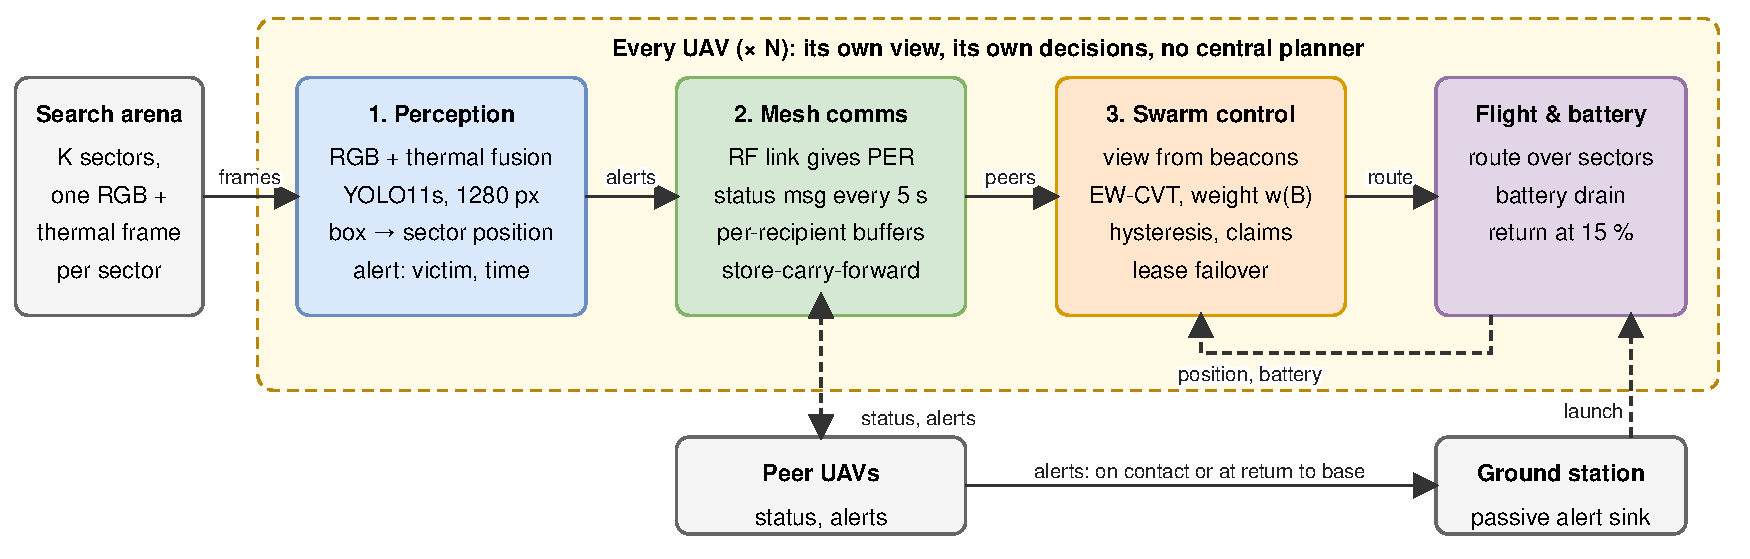
\includegraphics[width=\textwidth]{architecture.pdf}
\caption{System architecture. Solid arrows: data flow; dashed arrows: feedback, radio exchange and launch.}\label{fig:arch}
\end{figure}

\subsection{Multispectral Victim Detection}
The visible (RGB) and thermal long-wave infrared frames are stacked into a four-plane tensor, and the first convolution of the detector takes four input channels. The model is YOLO11s \cite{jocher2024yolo11} with an input size of 1280\,px, and the frames are $1280{\times}937$. It is trained on the NII-CU Multispectral Aerial Person Detection dataset \cite{speth2022} with a single person class. The thermal kernel is initialised from the pretrained red-channel kernel, which is the same technique as in the base paper, and training uses no colour jitter because colour has no meaning for a thermal plane.

\emph{Georeferencing.} The centre of a detected box is mapped linearly into the bounds of the sector in which the frame was taken, which gives a world coordinate. This is sector-based georeferencing and not a camera model, so the localisation error in the simulation measures the detector and not the optics.

Fig.~\ref{fig:pipeline} shows the path from the two cameras to an alert. \emph{Why early fusion.} Stacking the planes adds almost no computation to the first layer, so the detector is cheap enough for onboard use, and it lets the network use whichever plane is informative when the light is bad.


\begin{figure}[htbp]
\centering
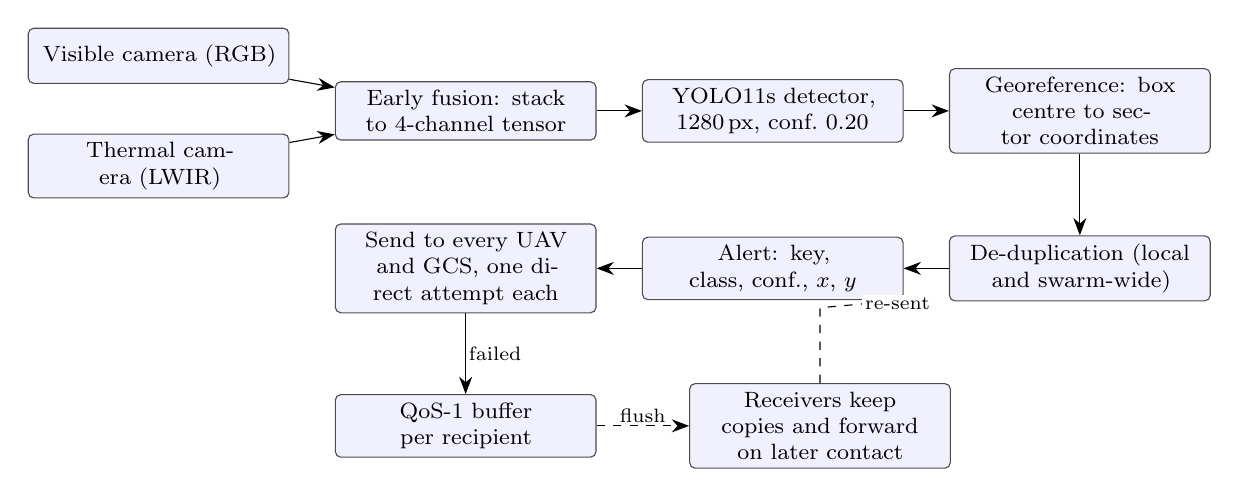
\begin{tikzpicture}
\node[blk](rgb)at(0,0.7){Visible camera (RGB)};
\node[blk](th)at(0,-0.7){Thermal camera (LWIR)};
\node[blk](fuse)at(3.9,0){Early fusion: stack to 4-channel tensor};
\node[blk](det)at(7.8,0){YOLO11s detector, 1280\,px, conf.\ 0.20};
\node[blk](geo)at(11.7,0){Georeference: box centre to sector coordinates};
\node[blk](dd)at(11.7,-2){De-duplication (local and swarm-wide)};
\node[blk](al)at(7.8,-2){Alert: key, class, conf., $x$, $y$};
\node[blk](snd)at(3.9,-2){Send to every UAV and GCS, one direct attempt each};
\node[blk](buf)at(3.9,-4){QoS-1 buffer per recipient};
\node[blk](fw)at(8.4,-4){Receivers keep copies and forward on later contact};
\draw[->](rgb)--(fuse);\draw[->](th)--(fuse);\draw[->](fuse)--(det);\draw[->](det)--(geo);
\draw[->](geo)--(dd);\draw[->](dd)--(al);\draw[->](al)--(snd);
\draw[->](snd)--node[lbl,right]{failed}(buf);
\draw[->,dashed](buf.east)--node[lbl,above]{flush}(fw.west);
\draw[->,dashed](fw.north)--(8.4,-2.5)--(al.south east)node[pos=0.5,lbl,right]{re-sent};
\end{tikzpicture}
\caption{Per-UAV pipeline from sensors to the operator: perception (top) and alert handling (bottom).}\label{fig:pipeline}
\end{figure}

\subsection{Wireless Channel Model}\label{sec:channel}
The path loss between two UAVs at distance $d$ follows a log-distance model with shadowing and obstruction:
\begin{equation}
PL(d)=PL(d_0)+10\,n\log_{10}\tfrac{d}{d_0}+X_\sigma+\Delta_{\text{obs}},
\end{equation}
where $PL(d_0)=20\log_{10}f_{\text{MHz}}-27.55$, $n=2.5$, $d_0=1$\,m, $X_\sigma$ is log-normal shadowing with $\sigma=4$\,dB, and $\Delta_{\text{obs}}=15$\,dB when the link is obstructed (a random 10\% chance beyond 50\,m) and 0 otherwise. The noise floor is $-90$\,dBm. The signal-to-noise ratio $\text{SNR}=P_{tx}-PL-N_0$ maps to a packet error rate: $\text{PER}=0$ above 25\,dB, $\text{PER}=1$ below 5\,dB, and in between
\begin{equation}
\text{PER}=1-\bigl(1+e^{-0.5(\text{SNR}-15)}\bigr)^{-1}.
\end{equation}
Arenas of 2\,km or more use 33\,dBm at 2.4\,GHz, which gives PER $\approx0.5$ at about 520\,m. Smaller arenas use 30\,dBm at 5\,GHz, with PER $\approx0.5$ at about 220\,m. In an arena that is several kilometres wide, the swarm is mostly disconnected in flight.

\subsection{Delay-Tolerant Alert Dissemination}
\subsubsection*{Alert generation and buffering}
When a UAV detects a victim, it makes one direct attempt to reach every other UAV and the GCS. Each failed copy is stored in a \emph{per-recipient QoS-1 buffer}, which is retained until it has been delivered. The buffer for a recipient is flushed when the link to that recipient has a PER below 0.2, which in practice happens when the UAV returns to base. A buffer with a capacity limit drops its oldest copy first.

\subsubsection*{Store-carry-forward relaying}
This is epidemic forwarding \cite{vahdat2000epidemic}. A UAV that \emph{receives} an alert also keeps a copy for each recipient that is not known to hold it, and it hands the copy over when it later meets that recipient with a good link. No UAV needs to be in the right place at the right moment, and an alert survives the loss of its finder. On contact, only the copies that the other side lacks are sent.

Fig.~\ref{fig:packet} shows what happens to one alert, step by step: the only network operation is a point-to-point attempt, and everything indirect is store-carry-forward.

\subsubsection*{Status messages}
Every 5\,s, each UAV broadcasts its position, its committed EW-CVT generator and weight, its state, the time at which its route should bring it home, its sector claims, and the set of sectors that it knows to be scanned. These messages are single-hop and are not buffered, since stale state is not worth delivering late. A receiver merges the scanned sets as grow-only sets, so the knowledge about coverage spreads transitively when UAVs meet.


\begin{figure}[htbp]
\centering
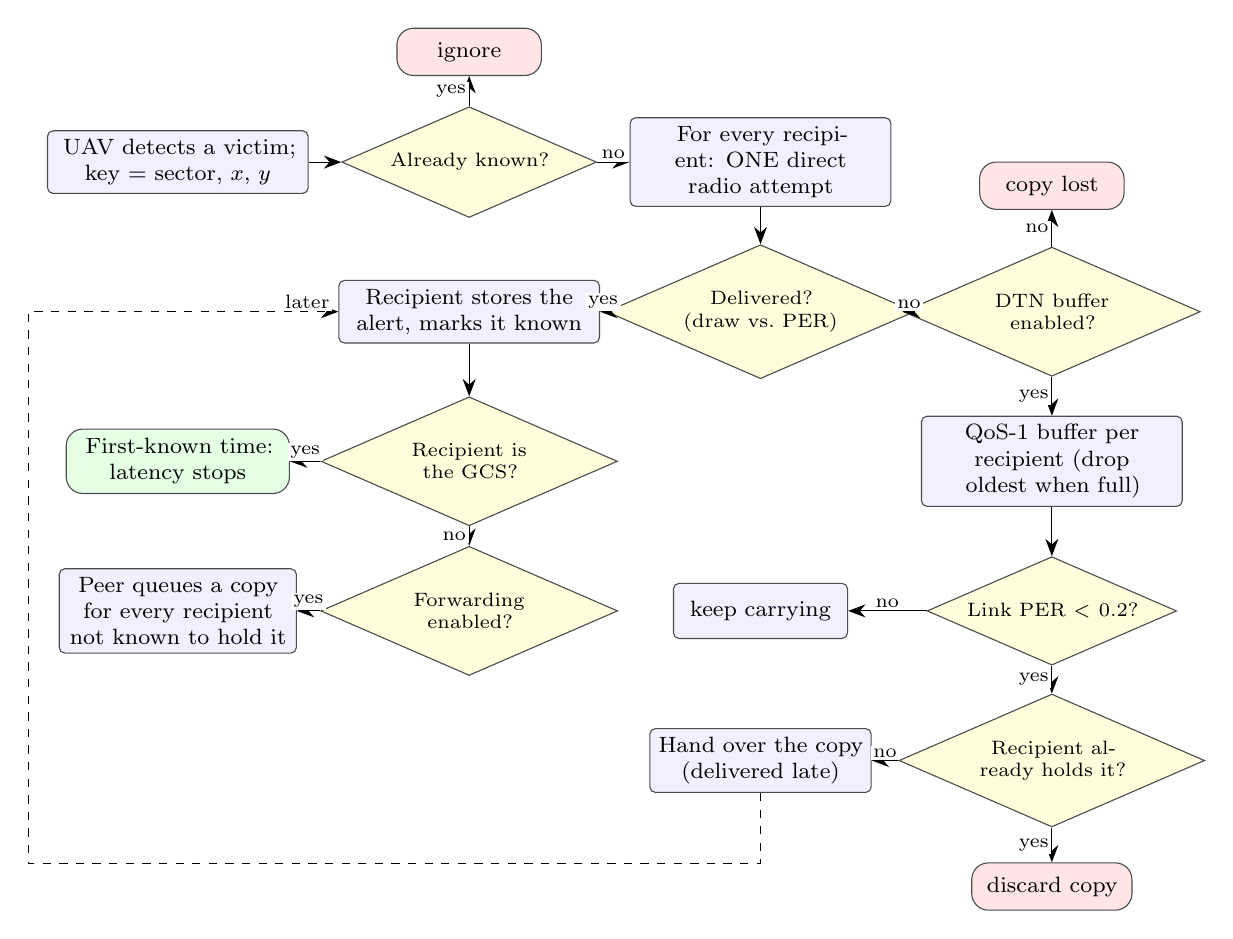
\begin{tikzpicture}[x=1cm,y=1cm]
\node[blk](det)at(0,0){UAV detects a victim; key = sector, $x$, $y$};
\node[dec](dup)at(3.7,0){Already known?};
\node[bad,text width=1.6cm](ig)at(3.7,1.4){ignore};
\node[blk](snd)at(7.4,0){For every recipient: ONE direct radio attempt};
\node[dec](per)at(7.4,-1.9){Delivered? (draw vs.\ PER)};
\node[blk](rx)at(3.7,-1.9){Recipient stores the alert, marks it known};
\node[dec](dtn)at(11.1,-1.9){DTN buffer enabled?};
\node[bad,text width=1.6cm](lost)at(11.1,-0.3){copy lost};
\node[dec](gcs)at(3.7,-3.8){Recipient is the GCS?};
\node[trm,text width=2.6cm](done)at(0,-3.8){First-known time: latency stops};
\node[dec](fwd)at(3.7,-5.7){Forwarding enabled?};
\node[blk,text width=2.8cm](carry)at(0,-5.7){Peer queues a copy for every recipient not known to hold it};
\node[blk](buf)at(11.1,-3.8){QoS-1 buffer per recipient (drop oldest when full)};
\node[dec](link)at(11.1,-5.7){Link PER $<0.2$?};
\node[blk,text width=2cm](wait)at(7.4,-5.7){keep carrying};
\node[dec](chk)at(11.1,-7.6){Recipient already holds it?};
\node[blk,text width=2.6cm](hand)at(7.4,-7.6){Hand over the copy (delivered late)};
\node[bad,text width=1.8cm](drop)at(11.1,-9.2){discard copy};
\draw[->](det)--(dup);\draw[->](dup)--node[lbl,left]{yes}(ig);\draw[->](dup)--node[lbl,above]{no}(snd);
\draw[->](snd)--(per);\draw[->](per)--node[lbl,above]{yes}(rx);\draw[->](per)--node[lbl,above]{no}(dtn);
\draw[->](rx)--(gcs);\draw[->](gcs)--node[lbl,above]{yes}(done);\draw[->](gcs)--node[lbl,left]{no}(fwd);
\draw[->](fwd)--node[lbl,above]{yes}(carry);
\draw[->](dtn)--node[lbl,left]{no}(lost);\draw[->](dtn)--node[lbl,left]{yes}(buf);
\draw[->](buf)--(link);\draw[->](link)--node[lbl,above]{no}(wait);\draw[->](link)--node[lbl,left]{yes}(chk);
\draw[->](chk)--node[lbl,above]{no}(hand);\draw[->](chk)--node[lbl,left]{yes}(drop);
\draw[->,dashed](hand.south)--++(0,-0.9)-|(-1.9,-1.9)--node[lbl,above,pos=0.9]{later}(rx.west);
\end{tikzpicture}
\caption{Packet delivery algorithm for a single alert: direct attempt, per-recipient buffering, store-carry-forward and contact-triggered hand-over.}\label{fig:packet}
\end{figure}

\subsection{Energy-Weighted Territory Partitioning (EW-CVT)}
Let $B_i$ be the battery level of UAV $i$ and $B_{\max}$ the capacity. The UAV has the weight
\begin{equation}
w_i=(B_i/B_{\max})^{\alpha}.
\end{equation}
A sector with centre $c_s$ is preferred by the UAV with the smallest weighted distance
\begin{equation}
d(s,i)=\frac{\lVert c_s-g_i\rVert^2}{\max(0.01,\,w_i)},\label{eq:pd}
\end{equation}
where $g_i$ is the committed generator of the UAV. For $\alpha=0$ the partition is a plain Voronoi diagram. A larger $\alpha$ shrinks the territory of low-battery UAVs, so the healthy UAVs do more of the work. The launch partition is the converged centroidal Voronoi tessellation, obtained by 15 Lloyd iterations: each generator is moved to the centroid of its cell, and this is repeated. Technically the result is a multiplicatively weighted Voronoi diagram and not a power diagram.

\subsection{Dual-Threshold Hysteresis}
Every 5\,s, each UAV computes the centroid $C_i^*$ that its cell should have. It does so over the peers that it \emph{believes} to be active, using their last advertised generators and weights. The UAV commits the new generator and weight only if
\begin{equation}
U_i=\big(\Delta B_i\ge\tau_\epsilon\ \wedge\ \lVert C_i^*-C_i\rVert\ge\tau_\delta\big)\ \vee\ \big(\mathcal N_i(t)\ne\mathcal N_i(t_k)\big),\label{eq:commit}
\end{equation}
with $\tau_\epsilon=2\%$ of $B_{\max}$, $\tau_\delta=5$\,m, and $\mathcal N_i$ the view of the live set held by the UAV. The first term requires both a real change in battery and a real movement of the centroid; the second term forces an update when the believed live set changes, for example after a failure. Fig.~\ref{fig:hyst-flow} shows the gate as a flowchart. Without this gate, noisy battery readings (here $\sigma=1.5$ points) would commit a new partition at every tick, and the route would change continuously.


\begin{figure}[htbp]
\centering
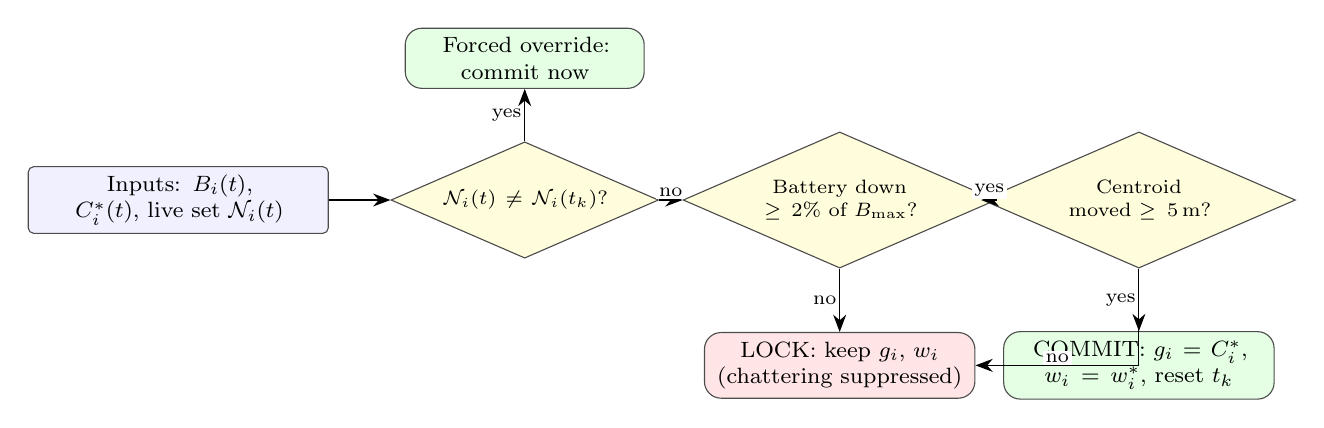
\begin{tikzpicture}
\node[blk,text width=3.6cm](in)at(0,0){Inputs: $B_i(t)$, $C_i^*(t)$, live set $\mathcal N_i(t)$};
\node[dec,text width=2.6cm](q1)at(4.4,0){$\mathcal N_i(t)\neq\mathcal N_i(t_k)$?};
\node[trm,text width=2.8cm](force)at(4.4,1.8){Forced override: commit now};
\node[dec,text width=2.6cm](q2)at(8.4,0){Battery down $\ge2\%$ of $B_{\max}$?};
\node[dec,text width=2.6cm](q3)at(12.2,0){Centroid moved $\ge5$\,m?};
\node[bad,text width=3.2cm](lock)at(8.4,-2.1){LOCK: keep $g_i$, $w_i$ (chattering suppressed)};
\node[trm,text width=3.2cm](com)at(12.2,-2.1){COMMIT: $g_i=C_i^*$, $w_i=w_i^*$, reset $t_k$};
\draw[->](in)--(q1);\draw[->](q1)--node[lbl,left]{yes}(force);\draw[->](q1)--node[lbl,above]{no}(q2);
\draw[->](q2)--node[lbl,above]{yes}(q3);\draw[->](q2)--node[lbl,left]{no}(lock);
\draw[->](q3)--node[lbl,left]{yes}(com);\draw[->](q3)|-node[lbl,pos=0.75,above]{no}(lock.east);
\end{tikzpicture}
\caption{Dual-threshold hysteresis gate with the topology override.}\label{fig:hyst-flow}
\end{figure}

\subsection{Claim-and-Yield Sector Assignment}
A UAV \emph{claims} a sector if it is the preferred owner by $d(s,i)$ (Eq.~\ref{eq:pd}) using committed values and no other UAV holds a valid claim on the sector. It keeps its existing claims unless a better claim (a smaller $d$, with ties broken by id) reaches it, and it then \emph{yields}. It may take over the claim of a peer only if it would arrive well before the advertised arrival time of that peer. A UAV that has no claims left takes the nearest unclaimed sector. Routes are greedy nearest-neighbour tours that end at the launch pad. Because claims are sticky, the number of sector flips stays low even when the views differ.

\subsection{Lease-Based Failure Detection and Failover}
In flight, silence tells a UAV nothing about a peer, because the peer may be out of range or it may have landed. Instead, each peer advertises the time at which its route should bring it home (its \emph{sortie lease}). A peer that is still missing \textit{slack} seconds after this time (60\,s by default) is \emph{suspected} to be lost, and its claims are released. Since a lost peer looks like one that landed quietly, released work is taken only by UAVs \emph{at base}, which have heard the landed peers. Landed UAVs listen for 10\,s, split the work among themselves by $d(s,i)$, and relaunch if the battery allows. A suspicion is withdrawn when the peer is heard again. A UAV aborts and returns at 15\% battery, and it is lost at 0\%.

Fig.~\ref{fig:failover} shows the sequence after a loss. The slack is a trade-off. A short slack detects a loss sooner but suspects more UAVs that are fine (a landed UAV looks crashed to a peer that is still in flight). A long slack is almost free of false alarms but delays the failover by minutes. Section~\ref{sec:results} quantifies this.


\begin{figure}[htbp]
\centering
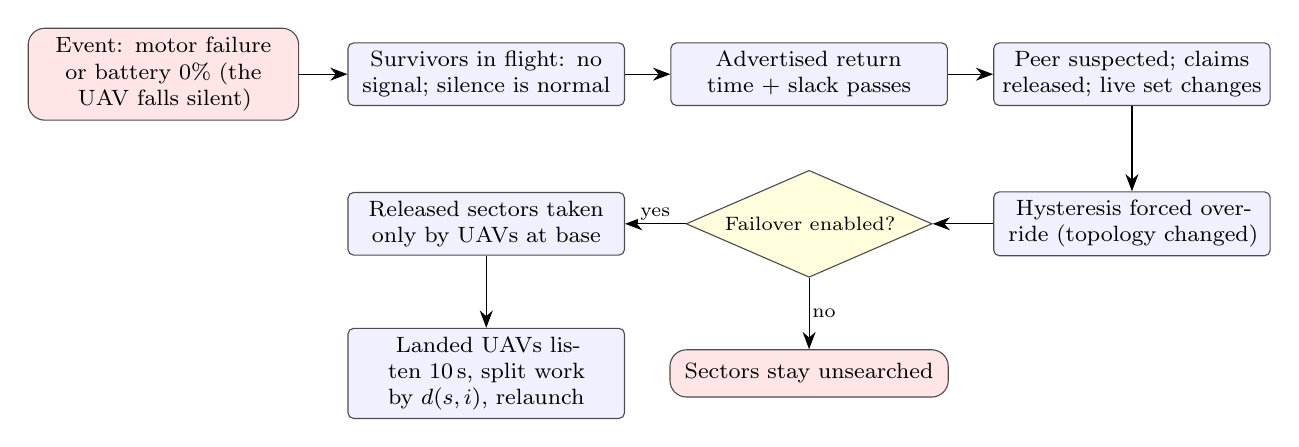
\begin{tikzpicture}
\node[bad,text width=3.2cm](ev)at(0,0){Event: motor failure or battery 0\% (the UAV falls silent)};
\node[blk,text width=3.3cm](si)at(4.1,0){Survivors in flight: no signal; silence is normal};
\node[blk,text width=3.3cm](le)at(8.2,0){Advertised return time + slack passes};
\node[blk,text width=3.3cm](su)at(12.3,0){Peer suspected; claims released; live set changes};
\node[blk,text width=3.3cm](ov)at(12.3,-1.9){Hysteresis forced override (topology changed)};
\node[dec,text width=2.5cm](fo)at(8.2,-1.9){Failover enabled?};
\node[blk,text width=3.3cm](ba)at(4.1,-1.9){Released sectors taken only by UAVs at base};
\node[blk,text width=3.3cm](sh)at(4.1,-3.8){Landed UAVs listen 10\,s, split work by $d(s,i)$, relaunch};
\node[bad,text width=3.3cm](un)at(8.2,-3.8){Sectors stay unsearched};
\draw[->](ev)--(si);\draw[->](si)--(le);\draw[->](le)--(su);\draw[->](su)--(ov);\draw[->](ov)--(fo);
\draw[->](fo)--node[lbl,above]{yes}(ba);\draw[->](fo)--node[lbl,right]{no}(un);\draw[->](ba)--(sh);
\end{tikzpicture}
\caption{Failure and failover sequence. A peer that only landed looks like a dead one until a UAV reaches base.}\label{fig:failover}
\end{figure}

\subsection{Control Loop}
Algorithm~\ref{alg:tick} and Fig.~\ref{fig:ctrl-flow} summarise one control tick of a UAV.

\begin{algorithm}[H]
\caption{Control tick of one UAV (every 5\,s).}\label{alg:tick}
\small
\begin{algorithmic}[1]
\State merge status messages received since the last tick into the view (peers, claims, scanned set)
\For{each peer $j$ overdue at base by more than \textit{slack}} mark $j$ suspected; release its claims
\EndFor
\State $\mathcal N_i\leftarrow$ self $\cup$ peers believed active (landed peers included only if self is at base)
\State read own battery $B_i$; $w_i^*\leftarrow(B_i/B_{\max})^{\alpha}$; $C_i^*\leftarrow$ EW-CVT centroid of my cell over $\mathcal N_i$
\If{$U_i$ (Eq.~\ref{eq:commit})} commit $g_i\leftarrow C_i^*$, $w_i\leftarrow w_i^*$
\EndIf
\State keep claims not beaten by a better claim; add free sectors that I prefer by $d(s,i)$
\If{no claims left} claim the nearest unclaimed sector; \textbf{if} at base, also share released work
\EndIf
\If{claims changed} rebuild route; advertise route ETA, claims and scanned set
\EndIf
\end{algorithmic}
\end{algorithm}


\begin{figure}[htbp]
\centering
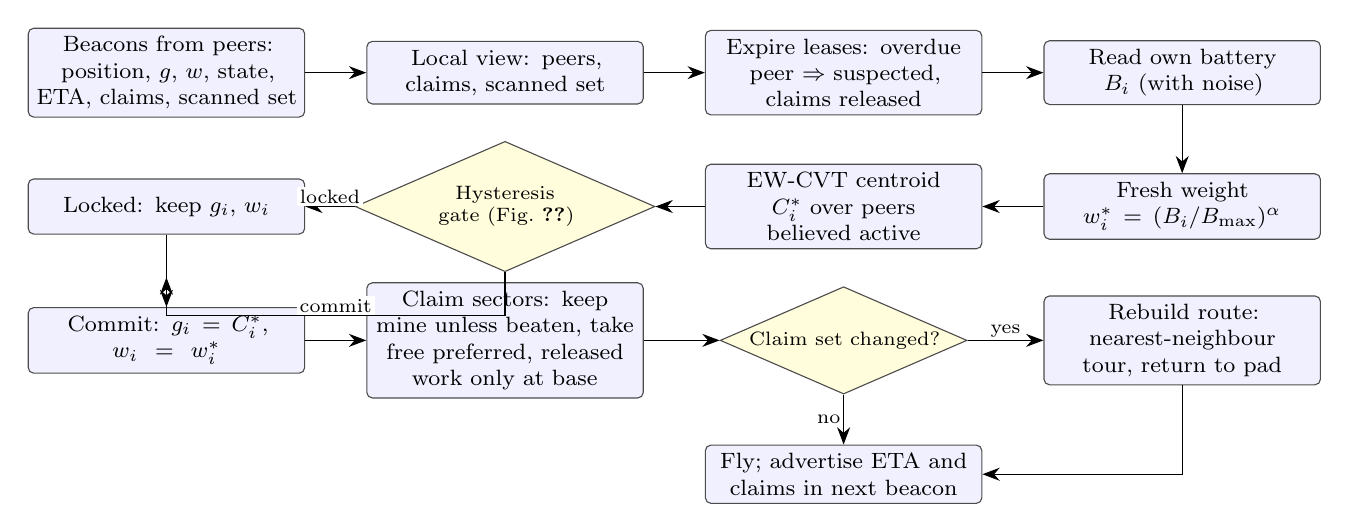
\begin{tikzpicture}
\node[blk,text width=3.3cm](bc)at(0,0){Beacons from peers: position, $g$, $w$, state, ETA, claims, scanned set};
\node[blk,text width=3.3cm](view)at(4.3,0){Local view: peers, claims, scanned set};
\node[blk,text width=3.3cm](exp)at(8.6,0){Expire leases: overdue peer $\Rightarrow$ suspected, claims released};
\node[blk,text width=3.3cm](meas)at(12.9,0){Read own battery $B_i$ (with noise)};
\node[blk,text width=3.3cm](w)at(12.9,-1.7){Fresh weight $w_i^*=(B_i/B_{\max})^{\alpha}$};
\node[blk,text width=3.3cm](cen)at(8.6,-1.7){EW-CVT centroid $C_i^*$ over peers believed active};
\node[dec,text width=2.4cm](gate)at(4.3,-1.7){Hysteresis gate (Fig.~\ref{fig:hyst-flow})};
\node[blk,text width=3.3cm](keep)at(0,-1.7){Locked: keep $g_i$, $w_i$};
\node[blk,text width=3.3cm](new)at(0,-3.4){Commit: $g_i=C_i^*$, $w_i=w_i^*$};
\node[blk,text width=3.3cm](cl)at(4.3,-3.4){Claim sectors: keep mine unless beaten, take free preferred, released work only at base};
\node[dec,text width=2.4cm](chg)at(8.6,-3.4){Claim set changed?};
\node[blk,text width=3.3cm](rt)at(12.9,-3.4){Rebuild route: nearest-neighbour tour, return to pad};
\node[blk,text width=3.3cm](adv)at(8.6,-5.1){Fly; advertise ETA and claims in next beacon};
\draw[->](bc)--(view);\draw[->](view)--(exp);\draw[->](exp)--(meas);\draw[->](meas)--(w);\draw[->](w)--(cen);\draw[->](cen)--(gate);
\draw[->](gate)--node[lbl,above]{locked}(keep);\draw[->](gate.south)--++(0,-0.55)-|node[lbl,pos=0.25,above]{commit}(0,-2.6);
\draw[->](keep)--(new);
\draw[->](new)--(cl);\draw[->](cl)--(chg);\draw[->](chg)--node[lbl,above]{yes}(rt);\draw[->](chg)--node[lbl,left]{no}(adv);\draw[->](rt)|-(adv);
\end{tikzpicture}
\caption{Control loop of one UAV, run every 5\,s from its own view only.}\label{fig:ctrl-flow}
\end{figure}

\subsection{Mission State Machine}
A UAV is in one of five states: \emph{TRANSIT} (flying to its first sector), \emph{SEARCHING} (scanning its claimed sectors), \emph{RETURNING} (heading home because its route is done or its battery has reached the 15\% reserve), \emph{LANDED} (at base, listening and sharing work), and \emph{CRASHED} (battery empty or failed). Fig.~\ref{fig:states} shows the transitions. The state is part of every status message. A landed UAV that has taken over released work and has enough battery relaunches into TRANSIT.


\begin{figure}[htbp]
\centering
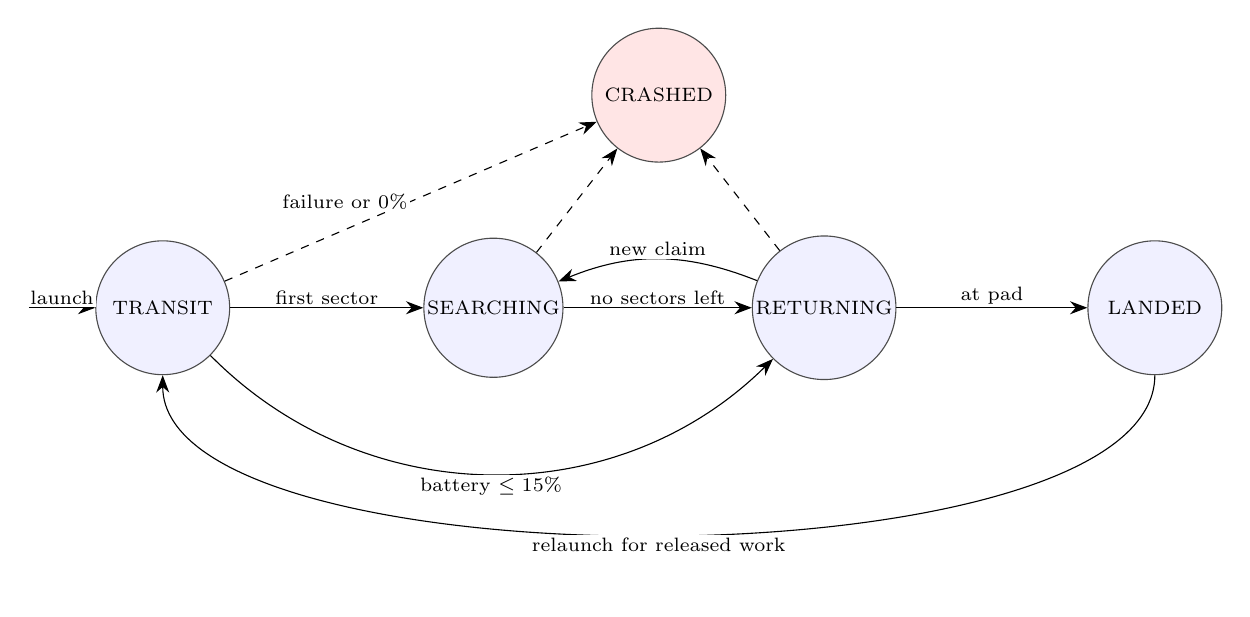
\begin{tikzpicture}[every node/.style={}]
\node[st](tr)at(0,0){TRANSIT};
\node[st](se)at(4.2,0){SEARCHING};
\node[st](re)at(8.4,0){RETURNING};
\node[st](la)at(12.6,0){LANDED};
\node[st,fill=red!10](cr)at(6.3,2.7){CRASHED};
\draw[->](-1.7,0)--node[lbl,above]{launch}(tr);
\draw[->](tr)--node[lbl,above]{first sector}(se);
\draw[->](se)--node[lbl,above]{no sectors left}(re);
\draw[->](re)to[bend right=22]node[lbl,above]{new claim}(se);
\draw[->](re)--node[lbl,above]{at pad}(la);
\draw[->](la)to[out=-90,in=-90,looseness=0.55]node[lbl,below]{relaunch for released work}(tr);
\draw[->](tr)to[bend right=45]node[lbl,below,pos=0.5]{battery $\le15\%$}(re);
\draw[->,dashed](tr)--node[lbl,left]{failure or 0\%}(cr);\draw[->,dashed](se)--(cr);\draw[->,dashed](re)--(cr);
\end{tikzpicture}
\caption{UAV state machine. A UAV keeps scanning sector after sector while SEARCHING. Dashed arrows lead to the absorbing CRASHED state; battery at or below 15\% also forces RETURNING from SEARCHING.}\label{fig:states}
\end{figure}

\subsection{Complexity}
A control tick involves $K$ sectors and $|\mathcal N_i|\le N$ peers. Evaluating $d(s,i)$ for every sector and peer costs $O(KN)$, the centroid computation another $O(K)$, and the greedy route $O(K_i^2)$ for $K_i$ claimed sectors. For $N=6$ and $K=25$ this is a few hundred operations every 5\,s, which is negligible for onboard hardware. A status message is $O(K+N)$ in size because of the scanned set and the claims.

%================================================================ 5
\section{Implementation}\label{sec:impl}
\subsection{Software Stack}
The project is written in Python. The detector uses PyTorch and Ultralytics YOLO11 \cite{jocher2024yolo11}. The project contains two layers.
\begin{itemize}
\item \textbf{Mission simulator} (\texttt{simulate\_swarm\_mission.py}, about 1,200 lines). A kinematic simulator with the classes \texttt{SimulatedUAV} and \texttt{SwarmSimulation}. It runs the full perception, communication and control logic described in Section~\ref{sec:design} on real dataset frames, and it is the source of all reported numbers.
\item \textbf{Flight and network platform} (\texttt{FlySim/}). A co-simulation platform derived from FlyNetSim \cite{baidya2018flynetsim} that couples ArduPilot software-in-the-loop aircraft with the ns-3 network simulator. It holds the swarm agent, the swarm network module, the hysteresis controller (\texttt{hysteresis\_controller.py}), the publish/subscribe layers for the UAVs and the GCS, and utilities for RF checks and demonstrations.
\end{itemize}

\subsection{Mission Simulator}
Each sector of the arena shows one frame of the dataset, and the labels of that frame are the ground truth for the sector. The simulator advances in steps of one second. In every step each UAV moves along its route, drains its battery, scans the sector below if it has arrived (which calls the detector or reads its cache), generates and attempts alerts, and, every 5\,s, runs a control tick and sends a status message. Links between UAVs and to the GCS are evaluated at every contact with the channel model of Section~\ref{sec:channel}. A failure is injected by marking a UAV as lost at a given time without any message.

To make 1,620 missions affordable, detections are cached: a frame has to be passed through the detector only once, and later missions that need the same frame read the result from the cache (\texttt{load\_detection\_cache} and \texttt{save\_detection\_cache}). A seed fixes the frame in each sector and every launch battery, so all variants of an experiment see identical worlds.

\subsection{Switches for Ablation}
Every component is a command-line switch, so an ablation changes one policy and nothing else. Table~\ref{tab:switch} lists the main switches.

\begin{table}[H]
\centering\small
\caption{Command-line switches of the mission simulator used for the experiments.}\label{tab:switch}
\begin{tabular}{p{3.8cm}p{10.4cm}}
\toprule
Switch & Effect\\
\midrule
\texttt{--drones, --arena, --grid} & Swarm size, arena width in metres, sectors per side\\
\texttt{--fail-drone, --fail-time} & UAV that is lost silently, and the time of the loss\\
\texttt{--alpha} & Exponent $\alpha$ of the EW-CVT weight\\
\texttt{--no-hysteresis} & Removes the dual-threshold gate\\
\texttt{--no-failover} & Released work is never taken over\\
\texttt{--static} & Fixed launch partition, no reassignment\\
\texttt{--no-dtn} & Removes the store-and-forward buffers\\
\texttt{--no-forwarding} & Removes store-carry-forward relaying\\
\texttt{--gcs-policy spray, --spray-copies} & Spray-and-wait relaying with $L$ copies\\
\texttt{--allocation auction} & Nearest-bidder allocation (all weights equal to 1)\\
\texttt{--buffer-cap} & Maximum buffered copies per UAV\\
\texttt{--batt-min, --batt-noise} & Lowest launch battery, and noise of battery readings\\
\texttt{--beacon-interval} & Seconds between status messages\\
\texttt{--lease-slack} & Seconds past the advertised return before a peer is suspected\\
\bottomrule
\end{tabular}
\end{table}

\subsection{Ablation and Reporting Pipeline}
The scripts in \texttt{ablation/} run the experiments and build the outputs: \texttt{run\_ablation.py} runs the missions and writes \texttt{results/ablation/runs.json}; \texttt{perception\_eval.py} evaluates the detector under the four input conditions; \texttt{make\_report.py}, \texttt{make\_readme.py} and \texttt{make\_paper\_assets.py} produce the HTML report, the results README, and the figures and tables of the paper. Every number in this report is generated by these scripts from the stored runs, which makes the study reproducible.

\subsection{Repository Layout}
\begin{itemize}
\item \texttt{simulate\_swarm\_mission.py}: mission simulator with perception, mesh and control.
\item \texttt{ablation/}: experiment runner, perception evaluation, report and paper generators.
\item \texttt{FlySim/}, \texttt{NetSim/}: ArduPilot and ns-3 co-simulation platform and its tools.
\item \texttt{results/}: stored runs, figures, headline table and the HTML report.
\item \texttt{docs/}: project overview, architecture diagrams, algorithms guide and how-to-run notes.
\item \texttt{paper/}: the conference paper (LaTeX), the draw.io architecture diagram and the Overleaf archive.
\item \texttt{report/}: this report.
\end{itemize}

%================================================================ 6
\section{Experimental Setup}\label{sec:setup}
\subsection{Simulation Environment}
Six UAVs search a $5\times5$\,km arena that is divided into 25 sectors. Each sector shows one frame of the NII-CU multispectral aerial person detection dataset \cite{speth2022}, whose labels serve as the ground truth (36 to 56 victims per world). The UAVs launch from a pad, fly at up to 50\,m/s in transit and 32\,m/s while searching, and drain 0.07 or 0.04\%/s of battery above or below 40\,m/s. The launch batteries are uniform between 20\% and 100\%, and the battery readings have a noise of $\sigma=1.5$ points. In the loss scenario, UAV~2 fails silently at $t=80$\,s. The network experiments use arenas of 1.5, 3 and 5\,km, and the scaling experiment uses 2 to 12 UAVs.

\subsection{Evaluation Metrics}

\begin{itemize}
\item \textbf{Coverage}: the share of sectors that were scanned at least once. \textbf{Mission time}: until completion or 1,500\,s.
\item \textbf{Precision} and \textbf{recall}: reported victims are matched to the ground truth within 15\,m (one-to-one), and recall is taken over all victims in the arena, so victims in unsearched sectors count against the system.
\item \textbf{Operator recall}: only the victims whose alert reached the GCS. \textbf{Alert latency}: the delay between detection and arrival at the GCS.
\item \textbf{Failover latency}: the time from the injected failure to the first claim of one of its sectors by a survivor.
\item \textbf{Duplicate scans}: sectors that were scanned more than once. \textbf{Sector flips}: claims given up to a better claim. \textbf{Route changes}: route rebuilds. \textbf{Commits}: updates approved by the hysteresis gate.
\item \textbf{Copies per alert}: the number of UAVs that hold a copy at the end, a measure of traffic cost.
\end{itemize}

\subsection{Baseline Methods}
Each baseline replaces one policy in the same simulator, so the missions, the radio model and the seeds are identical.
\begin{itemize}
\item \textbf{Forwarding.} \emph{Epidemic} (proposed): every UAV copies an alert to each UAV that it meets and that lacks one. \emph{Spray-and-wait} \cite{spyropoulos2005spray}: each alert gets $L=3$ copies, and the holder halves its copies at each hand-over and then waits to deliver directly. \emph{Buffer only}: each alert is carried home by its finder, with no relaying.
\item \textbf{Allocation.} \emph{EW-CVT} (proposed): the full scheme of Section~\ref{sec:design}. \emph{Auction without failover}: each sector is assigned to the nearest UAV (all weights equal to 1), and the sectors of a lost UAV are never reassigned. \emph{Static partition}: the launch partition is fixed, with no reassignment at all.
\end{itemize}



\subsection{Detector Conditions}
The shipped model is run on 150 held-out validation frames (IoU 0.5, confidence 0.25). The \emph{day} condition uses the frames unchanged. In the \emph{night} condition, the RGB plane is multiplied by 0.12 and noise ($\sigma=4$ grey levels) is added, which removes the visible cue and leaves thermal untouched. In the \emph{thermal washout} condition, which emulates people and background at nearly the same temperature, the thermal plane is compressed to 25\% of its contrast and noise ($\sigma=5$) is added, with RGB untouched. Both are synthetic degradations of daytime frames, not recorded data. In the \emph{RGB-only} and \emph{thermal-only} conditions, the other plane is set to zero. This is modality-masked inference of one fused network and not a comparison of separately trained models.



\subsection{Statistical Protocol}
Paired seeds are used: a seed fixes the frame in each sector and every launch battery, so each variant sees the same worlds. The study has 1,620 paired missions (81 configurations). We report paired differences with 95\% confidence intervals and claim no effect when an interval contains zero. Missions run until completion or 1,500\,s.

%================================================================ 7
\section{Results and Analysis}\label{sec:results}
\subsection{Detection Performance}
Table~\ref{tab:perc} shows the detector under the three conditions. The fused model reaches an AP50 of 99.8 in daylight. Fusion is about 11 points better than thermal only, so the visible plane adds information, while removing it at night costs only 5.5 points because thermal carries most of the detection. Thermal washout is the hardest case, because the network relies mainly on thermal: the recall falls to 0.39 while the precision stays at 0.99. The RGB-only case scores zero in every condition because the network was never trained without the thermal plane, so that number says nothing about the value of RGB, and trained single-modality baselines are still needed.

\begin{table}[H]
\centering\caption{Detection results on 150 held-out frames (AP in \%; precision and recall at confidence 0.25).}\label{tab:perc}
\resizebox{\textwidth}{!}{\begin{tabular}{lrrrrrrrrrrrr}
\toprule
& \multicolumn{4}{c}{Day} & \multicolumn{4}{c}{Night} & \multicolumn{4}{c}{Thermal washout}\\
\cmidrule(lr){2-5}\cmidrule(lr){6-9}\cmidrule(lr){10-13}
Input & AP50 & AP75 & Prec. & Rec. & AP50 & AP75 & Prec. & Rec. & AP50 & AP75 & Prec. & Rec.\\
\midrule
Fused RGB + thermal (proposed) & \textbf{99.8} & \textbf{85.8} & \textbf{0.993} & \textbf{0.989} & \textbf{94.3} & \textbf{58.3} & 0.916 & \textbf{0.869} & \textbf{61.8} & \textbf{25.1} & \textbf{0.991} & \textbf{0.386} \\
Thermal only (RGB zeroed) & 89.0 & 50.5 & 0.944 & 0.731 & 89.0 & 50.5 & \textbf{0.944} & 0.731 & 0.0 & 0.0 & 0.000 & 0.000 \\
\bottomrule
\end{tabular}
}
\end{table}

\subsubsection*{Comparison with the base paper}
Table~\ref{tab:speth} compares the daytime result with the base paper \cite{speth2022}, which reports YOLOv3 trained on the same dataset (Table~9 there, 485 aligned images with 891 people). Our fused YOLO11s model is ahead of their 4-channel model at AP50 (99.8 against 97.9) and at AP75 (85.8 against 76.9), and, like theirs, it is clearly ahead of the RGB-only and ensemble variants. The comparison is indicative only: we evaluate 150 of the 485 frames (275 people), the architecture (YOLO11s at 1280\,px against YOLOv3 at 960$\times$704) and the schedule differ, so part of the gap comes from the newer detector and not from the fusion. AP50:95 was not computed, and the checkpoint was selected on the same split. Latencies are not comparable (CPU here, a drone-class GPU in \cite{speth2022}).

\begin{table}[H]
\centering\small
\caption{Comparison with Speth et al.\ \cite{speth2022} (AP in \%). YOLO11s: 150 of 485 frames.}\label{tab:speth}
\begin{tabular}{llrr}
\toprule
Model & Input & AP50 & AP75\\
\midrule
YOLOv3 \cite{speth2022} & RGB & 92.4 & 44.5\\
YOLOv3 \cite{speth2022} & Thermal (FIR) & 97.5 & 72.7\\
YOLOv3 \cite{speth2022} & RGB + FIR ensemble & 97.3 & 54.7\\
YOLOv3 \cite{speth2022} & RGB + FIR, 4-channel & 97.9 & 76.9\\
YOLO11s (proposed) & RGB + FIR, 4-channel & \textbf{99.8} & \textbf{85.8}\\
\bottomrule
\end{tabular}
\end{table}

\begin{figure}[htbp]
\centering
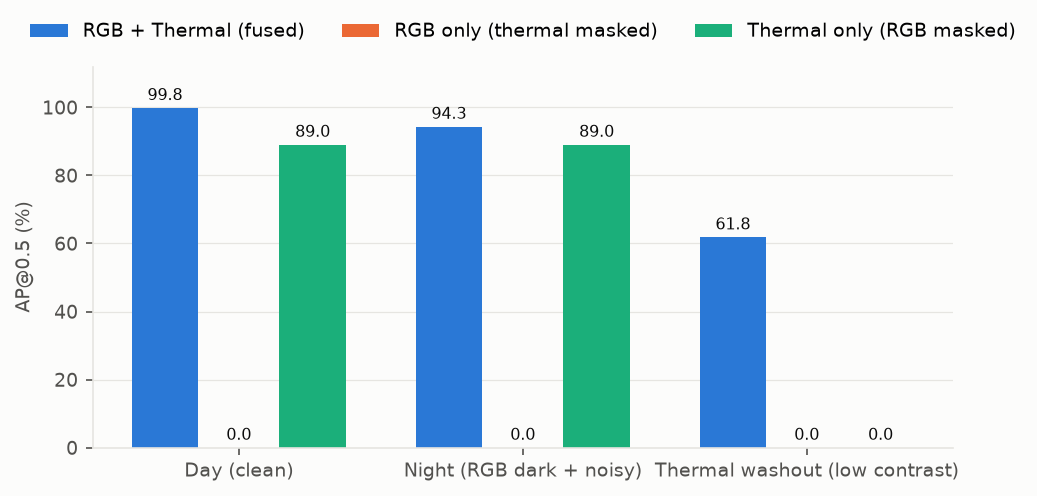
\includegraphics[width=0.6\textwidth]{detection_ap50_by_modality_and_condition.png}
\caption{AP50 of the detector by input modality and condition.}\label{fig:detap}
\end{figure}

\subsection{Reference Mission Performance}
Without a failure, the decentralised swarm covers 100\% of the arena in \pmsd{353}{31}\,s (mean $\pm$ s.d.). Precision, recall and F1 are all \pmsd{0.980}{0.015}, where the whole-arena recall counts the victims in unsearched sectors. The mean localisation error is \pmsd{1.45}{0.15}\,m, the first victim is detected after \pmsd{8.6}{7.2}\,s, and the operator learns of 100\% of the reports. No sector is scanned twice, and the minimum final battery is \pmsd{18.8}{8.3}\% of capacity.

\subsection{Ablation Study}
Table~\ref{tab:abl} gives the effect of removing each component, and Fig.~\ref{fig:covnet} shows the coverage over time and the network effect.

\begin{table}[H]
\centering\small
\caption{Ablation: paired change from the full system (mean $\pm$ 95\% CI). Network rows: 5\,km arena.}\label{tab:abl}
\begin{tabular}{p{6.6cm}rrr}
\toprule
Component removed: measure & Full & Ablated & Change\\
\midrule
Failover (UAV lost): coverage & 98.4\% & 87.4\% & $-11.0\pm2.6$\\
\quad whole-arena recall & 0.962 & 0.840 & $-0.122\pm0.032$\\
Hysteresis$^\dagger$: sector flips & 2.5 & 13.5 & $+11.0\pm3.5$\\
\quad route changes & 4.8 & 25.4 & $+20.6\pm6.4$\\
\quad mission time & 362\,s & 392\,s & $+30\pm25$\,s\\
EW weighting ($\alpha{=}0$): min.\ battery & 18.8\% & 17.9\% & $-0.8\pm0.7$\\
DTN buffer (5\,km): operator knows & 98.0\% & 3.4\% & $-94.7\pm1.2$\\
\quad swarm-wide consensus & 100\% & 22.1\% & $-77.9\pm1.3$\\
Forwarding (5\,km): alert latency & 103\,s & 109\,s & $+7\pm2$\,s\\
\bottomrule
\multicolumn{4}{l}{\scriptsize $^\dagger$ per-tick re-planning test configuration, $\sigma=2\%$ (see text).}
\end{tabular}
\end{table}

\begin{figure}[htbp]
\centering
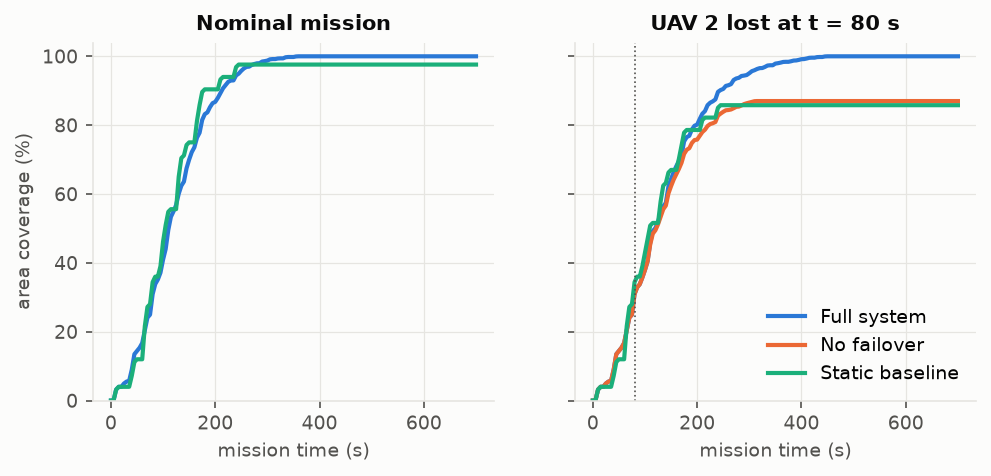
\includegraphics[width=0.49\textwidth]{coverage_over_time.png}\hfill
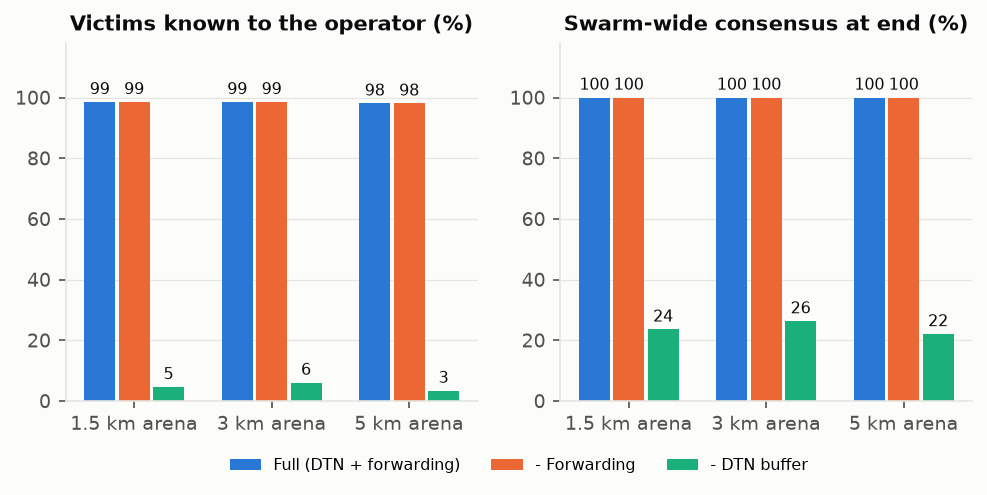
\includegraphics[width=0.49\textwidth]{network_ablation.png}
\caption{Left: coverage over time, nominal and with UAV~2 lost at 80\,s. Right: victims known to the operator, by arena size.}\label{fig:covnet}
\end{figure}

\subsubsection*{Failover}
Failover matters when a UAV is lost. The coverage after the loss is 98.4\% with failover and 87.4\% without it, since without failover the sectors of the lost UAV are never searched. The whole-arena recall falls from 0.962 to 0.840.

\subsubsection*{Hysteresis}
Hysteresis reduces churn but not flight time. In the full decentralised system it has almost no measurable effect, because the claims are already sticky (0.2 versus 0.4 sector flips), and this is a statement about the planner and not evidence that the gate is useless. It matters when a global planner recomputes the partitions from fresh readings at every tick. Table~\ref{tab:hyst} and Fig.~\ref{fig:hyst} show that hysteresis then cuts the commits about tenfold and the sector flips by a factor that grows with the noise, with the mission time unchanged within the intervals.

\begin{table}[H]
\centering\small
\caption{Hysteresis under battery-sensor noise (per-tick re-planning test).}\label{tab:hyst}
\begin{tabular}{rrrrrrr}
\toprule
Noise $\sigma$ (\%) & Flips ON & Flips OFF & Commits ON & Commits OFF & Time ON (s) & Time OFF (s)\\
\midrule
0 & 1.8 & 5.2 & 32 & 294 & 377 & 389\\
1 & 2.1 & 9.6 & 31 & 295 & 372 & 388\\
2 & 2.5 & 13.5 & 31 & 296 & 362 & 392\\
4 & 4.1 & 23.4 & 30 & 300 & 364 & 400\\
\bottomrule
\end{tabular}
\end{table}

\begin{figure}[htbp]
\centering
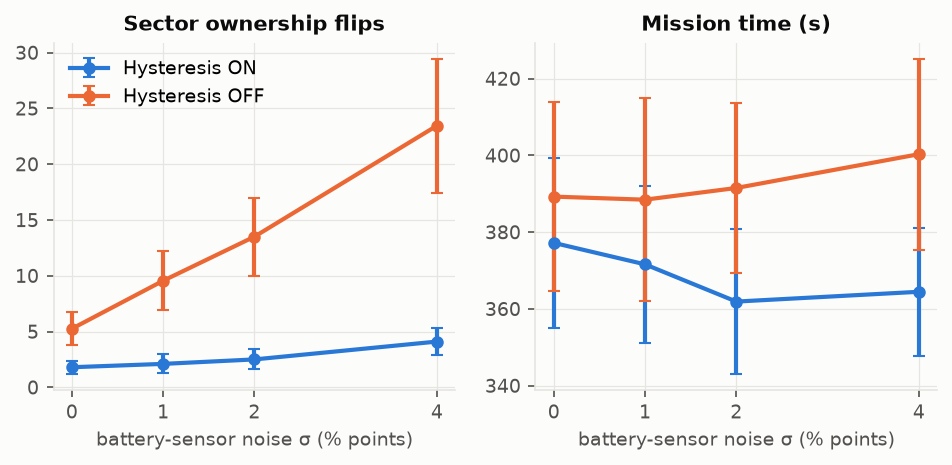
\includegraphics[width=0.62\textwidth]{hysteresis_vs_sensor_noise.png}
\caption{Hysteresis suppresses chattering as the sensor noise grows.}\label{fig:hyst}
\end{figure}

\subsubsection*{Energy weighting}
EW weighting is a trade-off. When $\alpha$ is swept from 0 to 3 (Table~\ref{tab:alpha}, Fig.~\ref{fig:alpha}), the minimum final battery rises from 15.6\% to 20.3\% and the low-battery aborts fall from 0.95 to 0.30 per mission, but the mission becomes longer (377 to 488\,s) because the healthy UAVs carry more of the work. Coverage is 100\% at every $\alpha$. The parameter is a dial between speed and energy safety, and not a free improvement.

\begin{table}[H]
\centering\small
\caption{Effect of the EW-CVT exponent $\alpha$ (mean $\pm$ 95\% CI).}\label{tab:alpha}
\begin{tabular}{rrrrr}
\toprule
$\alpha$ & Min.\ final battery (\%) & Mission time (s) & Coverage (\%) & Low-battery aborts\\
\midrule
0 & 15.6$\pm$6.5 & 377$\pm$94 & 100.0 & 0.95$\pm$0.89\\
0.5 & 16.1$\pm$7.1 & 349$\pm$42 & 100.0 & 0.90$\pm$0.85\\
1 & 16.7$\pm$7.0 & 358$\pm$27 & 100.0 & 0.90$\pm$0.85\\
2 & 18.3$\pm$6.9 & 427$\pm$71 & 100.0 & 0.45$\pm$0.76\\
3 & 20.3$\pm$8.8 & 488$\pm$114 & 100.0 & 0.30$\pm$0.47\\
\bottomrule
\end{tabular}
\end{table}

\begin{figure}[htbp]
\centering
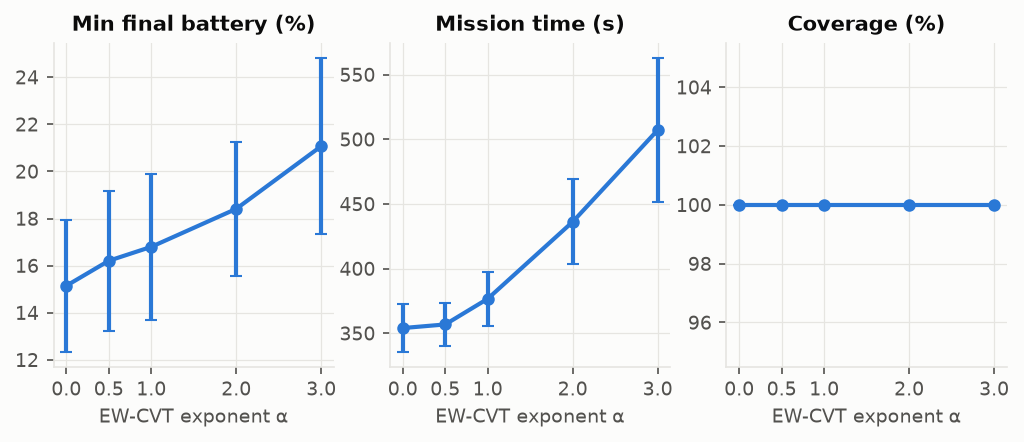
\includegraphics[width=0.62\textwidth]{alpha_sweep.png}
\caption{Time versus energy reserve as the exponent $\alpha$ is varied.}\label{fig:alpha}
\end{figure}

\subsection{Networking Results}
Under the radio model, direct links reach only a few hundred metres, so the swarm is mostly disconnected in flight and the first-attempt delivery to the GCS is only 3 to 6\% in every arena. Store-and-forward queues the alerts in the buffer of the UAV and flushes them when it returns to base, which turns a mostly offline swarm into one that the operator can rely on. Table~\ref{tab:net} shows that removing the buffer lowers the share of victims known to the operator from about 98\% to between 3\% and 6\%, and the swarm-wide consensus from 100\% to about 22 to 26\%.

\begin{table}[H]
\centering\small
\caption{Network ablation without a failure (mean $\pm$ 95\% CI).}\label{tab:net}
\begin{tabular}{llrrr}
\toprule
Arena & Variant & Operator recall & Alert latency (s) & Consensus\\
\midrule
1.5\,km & Full (DTN + forwarding) & 0.985$\pm$0.013 & 34$\pm$4 & 1.000\\
 & without forwarding & 0.985$\pm$0.013 & 41$\pm$5 & 1.000\\
 & without DTN buffer & 0.046$\pm$0.028 & -- & 0.236\\
3\,km & Full (DTN + forwarding) & 0.985$\pm$0.013 & 41$\pm$4 & 1.000\\
 & without forwarding & 0.985$\pm$0.013 & 59$\pm$7 & 1.000\\
 & without DTN buffer & 0.060$\pm$0.033 & -- & 0.263\\
5\,km & Full (DTN + forwarding) & 0.980$\pm$0.015 & 103$\pm$13 & 1.000\\
 & without forwarding & 0.980$\pm$0.015 & 109$\pm$12 & 1.000\\
 & without DTN buffer & 0.034$\pm$0.019 & -- & 0.221\\
\bottomrule
\end{tabular}
\end{table}

\subsubsection*{A UAV is lost before it returns}
If the finder is lost, its alerts reach the operator only if a peer that received them returns to base, and forwarding is what makes that possible. With the loss, forwarding raises the reports known to the operator from 0.976 to 0.989 at 1.5\,km and from 0.973 to 0.993 at 3\,km, and cuts the latency from 66 to 46\,s at 3\,km. At 5\,km the finder's own return is early enough that both variants reach 1.000.

\subsubsection*{Buffer capacity}
Epidemic forwarding stores many copies, so the capacity of the buffer matters. With a cap of 5, 15, 40 and 120 copies per UAV (3\,km, UAV lost), the reports known to the operator are 0.225, 0.415, 0.834 and 0.993, and the copies dropped fall from 389 to 11. A cap of about 120 copies loses nothing in this scenario, and a small cap fails badly.

\subsection{Comparison with Baseline Methods}
\subsubsection*{Forwarding policies}
Table~\ref{tab:dtn} and Fig.~\ref{fig:fwd} compare the forwarding policies. Epidemic forwarding has the lowest alert latency in every scenario, but it also holds the most copies. At 3\,km, its latency is 7.6$\pm$1.7\,s below spray-and-wait (paired difference with 95\% confidence interval) and 18\,s below buffering only, and it keeps about 1.9 more copies per alert than spray-and-wait. When UAV~2 is lost, the operator recall is 0.978 with epidemic forwarding, 0.967 with spray-and-wait and 0.958 with buffering only, and the latency gap to spray-and-wait grows to about 10\,s. Otherwise the operator recall is the same for all policies.

\begin{table}[H]
\centering\caption{Forwarding policies (mean $\pm$ 95\% CI). Lat.: alert latency; Copies: per alert.}\label{tab:dtn}
\resizebox{\textwidth}{!}{\begin{tabular}{lrrrrrrrr}
\toprule
& \multicolumn{2}{c}{1.5\,km} & \multicolumn{2}{c}{3\,km} & \multicolumn{2}{c}{5\,km} & \multicolumn{2}{c}{3\,km, UAV lost}\\
\cmidrule(lr){2-3}\cmidrule(lr){4-5}\cmidrule(lr){6-7}\cmidrule(lr){8-9}
Policy & Lat.\,(s) & Copies & Lat.\,(s) & Copies & Lat.\,(s) & Copies & Lat.\,(s) & Copies\\
\midrule
Epidemic (proposed) & \textbf{34.3{\scriptsize$\pm$2.1}} & 4.12 & \textbf{41.0{\scriptsize$\pm$1.8}} & 4.30 & \textbf{102.9{\scriptsize$\pm$6.0}} & 3.39 & \textbf{46.3{\scriptsize$\pm$3.3}} & 3.52 \\
Spray-and-wait & 36.4{\scriptsize$\pm$2.5} & 2.38 & 48.6{\scriptsize$\pm$2.2} & 2.37 & 106.3{\scriptsize$\pm$5.3} & 2.14 & 56.4{\scriptsize$\pm$4.8} & 2.29 \\
Buffer only & 41.4{\scriptsize$\pm$2.3} & 1.00 & 59.2{\scriptsize$\pm$3.3} & 1.00 & 109.5{\scriptsize$\pm$5.7} & 1.00 & 66.4{\scriptsize$\pm$4.3} & 1.04 \\
\bottomrule
\end{tabular}
}
\end{table}

\begin{figure}[htbp]
\centering
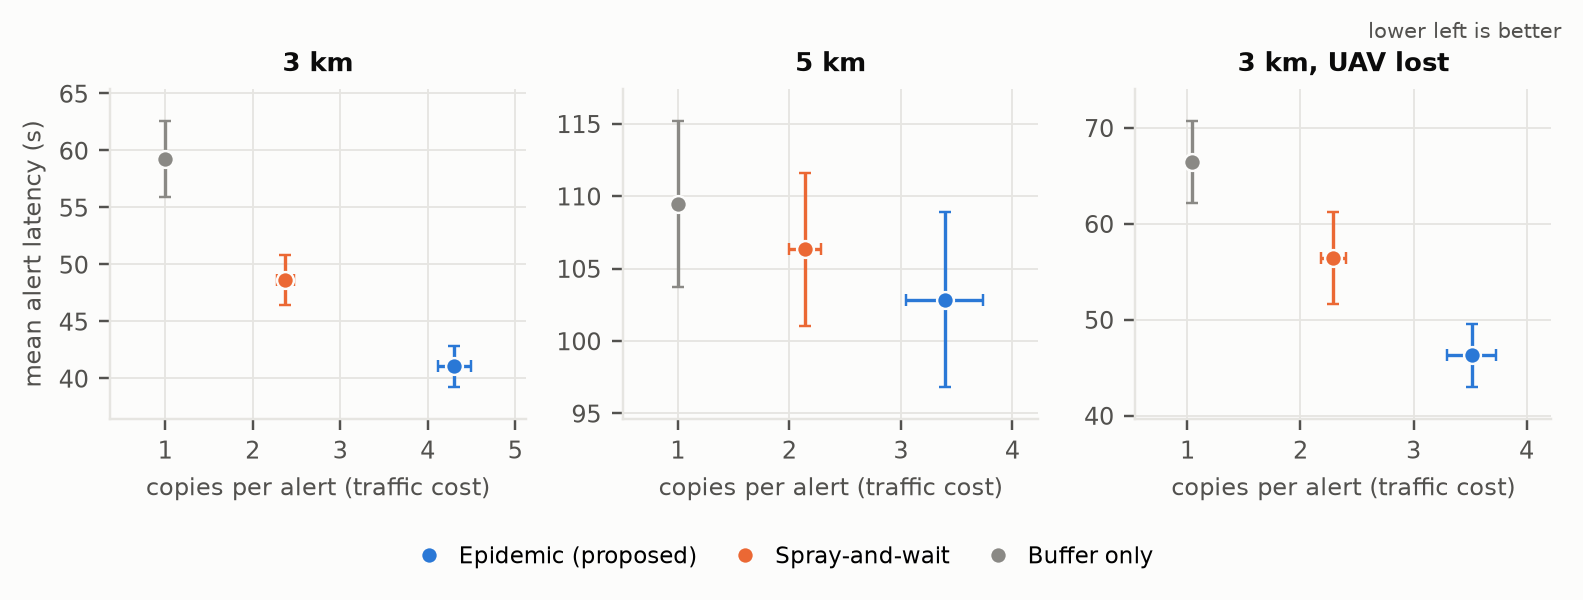
\includegraphics[width=0.58\textwidth]{forwarding_tradeoff.png}
\caption{Alert latency versus copies per alert (bars: 95\% CI).}\label{fig:fwd}
\end{figure}

\subsubsection*{Allocation policies}
Table~\ref{tab:alloc} and Fig.~\ref{fig:alloc} compare EW-CVT with a nearest-bidder auction without failover and with a static partition. Without a loss, all three reach full coverage. EW-CVT has no duplicate scans (0.00 against 0.90 and 0.10) and the highest minimum battery (18.8\% against 17.4\% and 17.9\%), but it is slower than the auction (353 against 334\,s). After a loss, the coverage is 98.4\% with failover against 89.2\% and 87.6\% for the auction and the static partition, and the arena recall is 0.96 against 0.87. The price is a longer mission, 554\,s against about 340\,s, because the survivors take over the work of the lost UAV. We credit the failover, and not the weighting, with the coverage gain.

\begin{table}[H]
\centering\caption{Allocation policies, nominal and with UAV~2 lost. Dup.: duplicate scans.}\label{tab:alloc}
\resizebox{\textwidth}{!}{\begin{tabular}{lrrrrrrrr}
\toprule
& \multicolumn{4}{c}{Nominal} & \multicolumn{4}{c}{UAV~2 lost}\\
\cmidrule(lr){2-5}\cmidrule(lr){6-9}
Policy & Cover.\,\% & Time (s) & Min.\,batt.\,\% & Dup. & Cover.\,\% & Time (s) & Min.\,batt.\,\% & Dup.\\
\midrule
EW-CVT (proposed) & \textbf{100.0} & 353 & \textbf{18.8} & \textbf{0.00} & \textbf{98.4} & 554 & 19.7 & 1.40 \\
Auction, no failover & \textbf{100.0} & \textbf{334} & 17.4 & 0.90 & 89.2 & \textbf{336} & 20.0 & 0.75 \\
Static partition & \textbf{100.0} & 364 & 17.9 & 0.10 & 87.6 & 353 & \textbf{20.3} & \textbf{0.30} \\
\bottomrule
\end{tabular}
}
\end{table}

\begin{figure}[htbp]
\centering
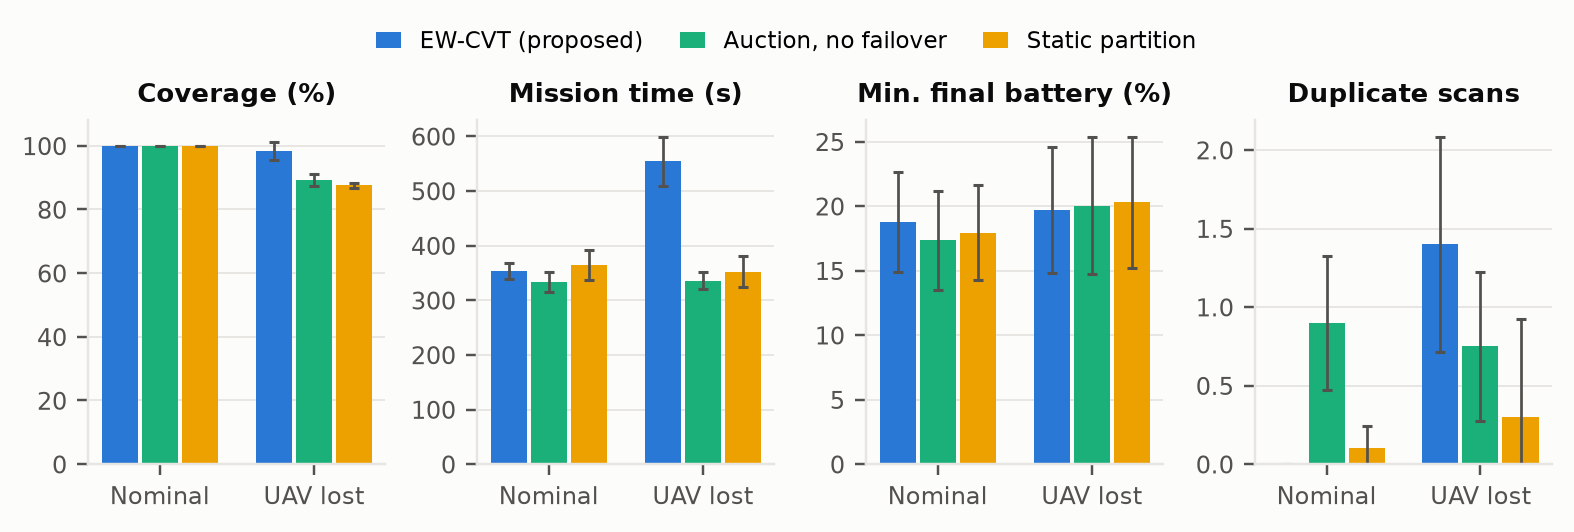
\includegraphics[width=0.58\textwidth]{allocation_baselines.png}
\caption{Allocation policies: coverage, time, battery and duplicates (bars: 95\% CI).}\label{fig:alloc}
\end{figure}

\subsection{Failure Recovery Analysis}
Table~\ref{tab:dec} shows the behaviour of the swarm when UAV~2 is lost. The survivors cannot know that the UAV is gone until it is overdue at base, so failover takes minutes. It takes 231\,s on average at 5\,km, 143\,s at 3\,km and 102\,s at 1.5\,km, and the shorter times in smaller arenas follow from the UAVs meeting more often. The coverage stays at 98.4\% or above, but the mission at 5\,km grows from 353\,s to 554\,s. In a few seeds, sectors stay unsearched because the survivors lack the battery for a second sortie by the time they learn of the loss.

\begin{table}[H]
\centering\small
\caption{Recovery after the loss of UAV~2. Failover: time to the first claim of its sectors.}\label{tab:dec}
\begin{tabular}{lrrr}
\toprule
Scenario & Cover.\,\% & Time (s) & Failover (s)\\
\midrule
5\,km, no loss & 100.0 & 353 & n/a \\
5\,km, loss & 98.4 & 554 & 231 \\
3\,km, loss & 99.0 & 326 & 143 \\
1.5\,km, loss & 99.2 & 171 & 102 \\
\bottomrule
\end{tabular}

\end{table}

\subsubsection*{Lease slack}
The slack trades detection speed against false alarms (Table~\ref{tab:slack}, Fig.~\ref{fig:slack}). For slack values of 20, 60, 120 and 240\,s, the mean failover latency is 192, 231, 293 and 411\,s, and the wrong suspicions fall from 11.2 of 15.6 to 0.4 of 4.7 per mission. Most suspicions concern UAVs that were fine (a landed UAV looks crashed to a peer in flight), but they cost little because released work is taken only at base.

\begin{table}[H]
\centering\small
\caption{Effect of the lease slack after the loss of UAV~2 (5\,km).}\label{tab:slack}
\begin{tabular}{rrrrrr}
\toprule
Slack (s) & Failover (s) & Mission time (s) & Coverage (\%) & Duplicates & Wrong suspicions\\
\midrule
20 & 192$\pm$43 & 518$\pm$101 & 98.6 & 1.1 & 11.2 of 15.6\\
60 & 231$\pm$43 & 554$\pm$97 & 98.4 & 1.4 & 8.3 of 12.6\\
120 & 293$\pm$42 & 587$\pm$102 & 98.6 & 0.7 & 3.6 of 8.0\\
240 & 411$\pm$43 & 698$\pm$128 & 98.6 & 0.7 & 0.4 of 4.7\\
\bottomrule
\end{tabular}
\end{table}

\begin{figure}[htbp]
\centering
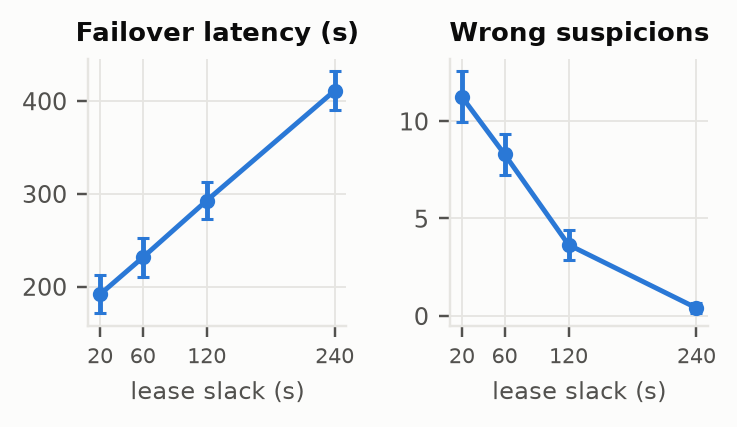
\includegraphics[width=0.58\textwidth]{lease_slack_tradeoff.png}
\caption{Lease slack: failover latency against wrong suspicions.}\label{fig:slack}
\end{figure}

\subsubsection*{Status interval}
The status interval hardly affects the mission time (532 to 629\,s for 2 to 60\,s) until it approaches the duration of a contact. At 60\,s the coverage drops to 96.4\% and the duplicate scans rise from 0.6 to 2.6, while the number of control messages that are delivered falls from about 1,850 to 80.

\subsection{Scaling with Swarm Size}
Fig.~\ref{fig:scale} and Table~\ref{tab:scale} show the effect of the swarm size in the 5\,km arena. The mission time falls from 554\,s with 2 UAVs to 261\,s with 12, and the energy used per UAV falls from 24.9\% to 11.1\%, while the recall stays at 0.980. The speed-up is sublinear because the transit from the base is a fixed cost. The small non-monotonicity between 4 and 6 UAVs is probably an artefact of how the starting territories are laid out (corners for up to 4 UAVs, a ring for more), but this has not been verified.

\begin{table}[H]
\centering\small
\caption{Scaling with swarm size.}\label{tab:scale}
\begin{tabular}{rrrr}
\toprule
Swarm size & Mission time (s) & Mean energy used per UAV (\%) & Recall (arena)\\
\midrule
2 & 554 & 24.9 & 0.980\\
4 & 329 & 16.9 & 0.980\\
6 & 337 & 12.9 & 0.980\\
8 & 296 & 12.2 & 0.980\\
12 & 261 & 11.1 & 0.980\\
\bottomrule
\end{tabular}
\end{table}

\begin{figure}[htbp]
\centering
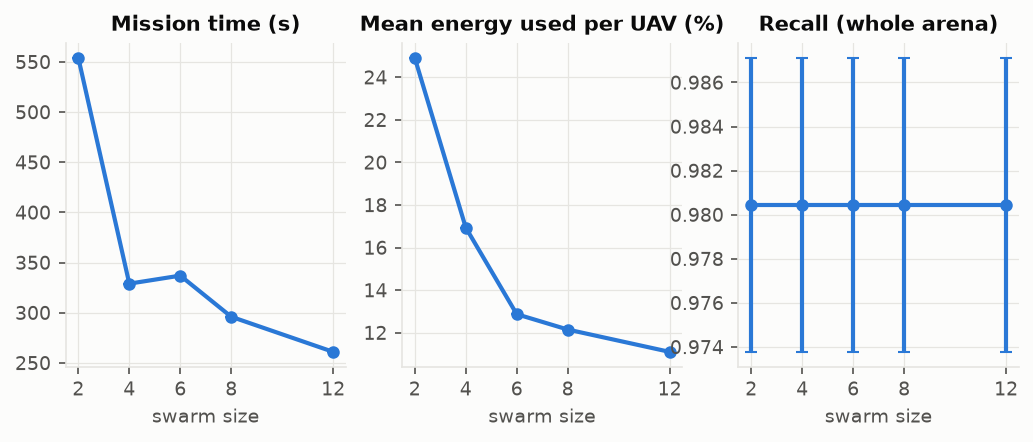
\includegraphics[width=0.62\textwidth]{scaling.png}
\caption{Mission time and energy per UAV as the swarm grows.}\label{fig:scale}
\end{figure}

%================================================================ 8
\section{Discussion}\label{sec:disc}
\subsection{What the Evidence Supports}
Two conclusions are clearly supported. First, a sparsely connected swarm needs buffering: without the per-recipient buffers the operator knows of only 3 to 6\% of the victims, and with them about 98\%. Second, losing a UAV costs coverage unless the others take over its work, with a delay that is set by how long the survivors need to learn of the loss. Hysteresis matters only where partitions are recomputed from noisy readings at every tick, and energy weighting buys reserve at the price of speed.

\subsection{The Price of Decentralisation}
The decentralised design is robust, but it is not free. A central planner that knew at once that a UAV was lost could reassign its sectors immediately. The UAVs here cannot know, because in flight silence is normal, and so they wait for the lease of the lost UAV to expire and for the survivors to be at base. This makes the failover latency minutes and extends the mission by about 200\,s at 5\,km. The experiments show the shape of the trade-off: a shorter slack buys speed at the cost of wrong suspicions, which are cheap here because released work is taken only at base.

\subsection{Epidemic versus Bounded Forwarding}
Epidemic forwarding gives the lowest latency because every encounter spreads the alert, and it uses the most copies for the same reason. Spray-and-wait bounds the copies at $L=3$ and pays a few seconds of latency; buffering only has a single copy and the highest latency. For a search and rescue mission, where the cost of a delayed alert is a victim who waits longer and the cost of a copy is a few bytes of storage, epidemic forwarding is the natural choice, provided that the buffer cap is large enough (Section~\ref{sec:results}).

\subsection{Perception under Degraded Conditions}
The fused detector keeps a high precision in every condition (0.92 to 0.99), and its weak point is the recall in thermal washout (0.39). In that condition the visible plane could help, but the network has learned to lean on thermal. This suggests training with random modality dropout, which would teach the network to use whichever plane is informative.

%================================================================ 9
\section{Limitations and Future Work}\label{sec:limits}
\subsection{Limitations}
\begin{enumerate}
\item \textbf{Simulation only.} The simulator is kinematic, with constant speeds, linear battery drain and no wind, and the network results depend on the radio model. No physical UAV has flown.
\item \textbf{Static frames.} Each sector shows one static dataset frame, so the mission-level precision and recall mostly reflect the detector on these frames and the sectors that were visited. The training and validation frames come from the same site, so the absolute numbers are probably optimistic.
\item \textbf{Perception ablation.} It masks one plane of a single fused network. Separately trained RGB-only and thermal-only detectors are needed for a proper modality comparison, and the night and washout conditions are synthetic.
\item \textbf{Simplified decentralisation.} The UAVs launch together and share the initial partition, status messages are single-hop, alerts are addressed to every UAV whether alive or not, and forwarding reads the holdings of the receiver instead of simulating the exchange on contact.
\item \textbf{Failure-detector design.} The lease detector is one of several possible designs and has not been compared with the others, and the 15\% reserve and the noise levels are scenario assumptions. The comparison with the base paper is indicative only (Section~\ref{sec:results}).
\end{enumerate}

\subsection{Future Work}
\begin{itemize}
\item Train separate RGB-only and thermal-only detectors (and a fused one with modality dropout) and evaluate on the full 485-frame set with AP50:95.
\item Compare complete prior-work stacks across a sweep of network connectivity.
\item Let status messages carry third-party state, so that failure detection does not wait for an overdue return.
\item Add a camera model, wind and richer energy models, and run the control logic on the ArduPilot and ns-3 platform and finally on real hardware.
\end{itemize}

%================================================================ 10
\section{Conclusion}\label{sec:concl}
This project presented a decentralised search-and-rescue system for swarms that are mostly out of radio contact. It integrates early-fusion RGB and thermal perception, a delay-tolerant mesh with store-carry-forward relaying, and an energy-aware coordination layer without a central planner. Over 1,620 paired simulated missions, buffering was the largest effect that we measured, raising the share of victims known to the operator from 3.4\% to 98\% in a 5\,km arena. Failover recovers 11 points of coverage after a UAV is lost, and epidemic relaying delivers alerts 7.6\,s sooner than spray-and-wait at 3\,km, at the price of about two more copies of each alert. The price of decentralisation is a failover latency of minutes, because no UAV can know of a loss before the missing one is overdue at base. The fused detector reaches an AP50 of 99.8 in daylight and 94.3 at night, and its main weakness is the recall under thermal washout. All results come from simulation, and the unfavourable results and the limits of the study have been reported together with the favourable ones.

\clearpage
\addcontentsline{toc}{section}{References}
\renewcommand{\refname}{References}
\begin{thebibliography}{99}
\bibitem{speth2022} Speth, S., Gon\c{c}alves, A., Rigault, B., \textit{et al.}: `Deep learning with RGB and thermal images onboard a drone for monitoring operations', \textit{J. Field Robot.}, 2022, \textbf{39}, (6), pp. 840--868 (dataset: \nolinkurl{https://www.nii-cu-multispectral.org}).
\bibitem{gerkey2004} Gerkey, B.P., Matari\'c, M.J.: `A formal analysis and taxonomy of task allocation in multi-robot systems', \textit{Int. J. Robot. Res.}, 2004, \textbf{23}, (9), pp. 939--954.
\bibitem{grontved2023} Gr{\o}ntved, K.A.R., Lundquist, U.P.S., Christensen, A.L.: `Decentralized multi-UAV trajectory task allocation in search and rescue applications'. Proc. IEEE Int. Conf. Advanced Robotics, Abu Dhabi, UAE, December 2023, pp. 35--41.
\bibitem{olfatisaber2007} Olfati-Saber, R., Fax, J.A., Murray, R.M.: `Consensus and cooperation in networked multi-agent systems', \textit{Proc. IEEE}, 2007, \textbf{95}, (1), pp. 215--233.
\bibitem{cortes2004coverage} Cort\'es, J., Mart\'inez, S., Karatas, T., \textit{et al.}: `Coverage control for mobile sensing networks', \textit{IEEE Trans. Robot. Autom.}, 2004, \textbf{20}, (2), pp. 243--255.
\bibitem{du1999cvt} Du, Q., Faber, V., Gunzburger, M.: `Centroidal Voronoi tessellations: applications and algorithms', \textit{SIAM Rev.}, 1999, \textbf{41}, (4), pp. 637--676.
\bibitem{chandra1996} Chandra, T.D., Toueg, S.: `Unreliable failure detectors for reliable distributed systems', \textit{J. ACM}, 1996, \textbf{43}, (2), pp. 225--267.
\bibitem{hayashibara2004} Hayashibara, N., D\'efago, X., Yared, R., \textit{et al.}: `The $\varphi$ accrual failure detector'. Proc. IEEE Symp. Reliable Distributed Systems, Florianopolis, Brazil, October 2004, pp. 66--78.
\bibitem{fall2003dtn} Fall, K.: `A delay-tolerant network architecture for challenged internets'. Proc. ACM SIGCOMM, Karlsruhe, Germany, August 2003.
\bibitem{vahdat2000epidemic} Vahdat, A., Becker, D.: `Epidemic routing for partially connected ad hoc networks'. Technical Report CS-2000-06, Duke University, 2000.
\bibitem{spyropoulos2005spray} Spyropoulos, T., Psounis, K., Raghavendra, C.S.: `Spray and wait: an efficient routing scheme for intermittently connected mobile networks'. Proc. ACM SIGCOMM Workshop on Delay-Tolerant Networking, Philadelphia, USA, August 2005.
\bibitem{hwang2015kaist} Hwang, S., Park, J., Kim, N., \textit{et al.}: `Multispectral pedestrian detection: benchmark dataset and baseline'. Proc. IEEE Conf. Computer Vision and Pattern Recognition, Boston, USA, June 2015.
\bibitem{jia2021llvip} Jia, X., Zhu, C., Li, M., \textit{et al.}: `LLVIP: a visible-infrared paired dataset for low-light vision'. Proc. IEEE/CVF Int. Conf. Computer Vision Workshops, Montreal, Canada, October 2021.
\bibitem{goodrich2008} Goodrich, M.A., Morse, B.S., Gerhardt, D., \textit{et al.}: `Supporting wilderness search and rescue using a camera-equipped mini UAV', \textit{J. Field Robot.}, 2008, \textbf{25}, (1--2), pp. 89--110.
\bibitem{burgard2005} Burgard, W., Moors, M., Stachniss, C., \textit{et al.}: `Coordinated multi-robot exploration', \textit{IEEE Trans. Robot.}, 2005, \textbf{21}, (3), pp. 376--386.
\bibitem{giacomossi2026} Giacomossi, L., \textit{et al.}: `Market-based replanning for safety-critical UAV swarms in search and rescue missions', arXiv:2606.01970, 2026.
\bibitem{bekmezci2013} Bekmezci, \.I., Sahingoz, O.K., Temel, \c{S}.: `Flying ad-hoc networks (FANETs): a survey', \textit{Ad Hoc Netw.}, 2013, \textbf{11}, (3), pp. 1254--1270.
\bibitem{redmon2016yolo} Redmon, J., Divvala, S., Girshick, R., \textit{et al.}: `You only look once: unified, real-time object detection'. Proc. IEEE Conf. Computer Vision and Pattern Recognition, Las Vegas, USA, June 2016.
\bibitem{jocher2024yolo11} Jocher, G., Qiu, J.: `Ultralytics YOLO11', 2024, \nolinkurl{https://github.com/ultralytics/ultralytics}.
\bibitem{lloyd1982} Lloyd, S.P.: `Least squares quantization in PCM', \textit{IEEE Trans. Inf. Theory}, 1982, \textbf{28}, (2), pp. 129--137.
\bibitem{aurenhammer1987power} Aurenhammer, F.: `Power diagrams: properties, algorithms and applications', \textit{SIAM J. Comput.}, 1987, \textbf{16}, (1), pp. 78--96.
\bibitem{kwok2007} Kwok, A., Mart\'inez, S.: `Energy-balancing cooperative strategies for sensor deployment'. Proc. IEEE Conf. Decision and Control, New Orleans, USA, December 2007, pp. 6136--6141.
\bibitem{munir2024} Munir, A., Dutta, A., Parasuraman, R.: `Energy-aware coverage planning for heterogeneous multi-robot system', arXiv:2411.02230, 2024.
\bibitem{gray1989} Gray, C.G., Cheriton, D.R.: `Leases: an efficient fault-tolerant mechanism for distributed file cache consistency'. Proc. ACM Symp. Operating Systems Principles, Litchfield Park, USA, December 1989, pp. 202--210.
\bibitem{kosaka2023dmlt} Kosaka, K., Noda, Y., Yokotani, T., \textit{et al.}: `Implementation and evaluation of the control mechanism among distributed MQTT brokers', \textit{IEEE Access}, 2023, \textbf{11}, doi: 10.1109/ACCESS.2023.3335273.
\bibitem{rappaport2002wireless} Rappaport, T.S.: `Wireless communications: principles and practice' (Prentice Hall, 2002, 2nd edn.).
\bibitem{baidya2018flynetsim} Baidya, S., Shaikh, Z., Levorato, M.: `FlyNetSim: an open source synchronized UAV network simulator based on ns-3 and Ardupilot'. Proc. ACM Int. Conf. Modeling, Analysis and Simulation of Wireless and Mobile Systems, Montreal, Canada, October 2018, pp. 37--45.
\end{thebibliography}

\end{document}
